%%%%%%%%%%%%%%%%%%%% author.tex %%%%%%%%%%%%%%%%%%%%%%%%%%%%%%%%%%%
%
% sample root file for your "contribution" to a contributed volume
%
% Use this file as a template for your own input.
%
%%%%%%%%%%%%%%%% Springer %%%%%%%%%%%%%%%%%%%%%%%%%%%%%%%%%%

% RECOMMENDED %%%%%%%%%%%%%%%%%%%%%%%%%%%%%%%%%%%%%%%%%%%%%%%%%%%
\documentclass[graybox]{svmult}

% choose options for [] as required from the list
% in the Reference Guide

%\usepackage{mathptmx}       % selects Times Roman as basic font
% Much better times roman fonts are obtained with the following 3 lines.
\usepackage{newtxmath,newtxtext}
\DeclareSymbolFont{operators}{OT1}{ntxtlf}{m}{n}
\SetSymbolFont{operators}{bold}{OT1}{ntxtlf}{b}{n}
\usepackage{helvet}         % selects Helvetica as sans-serif font
\usepackage{courier}        % selects Courier as typewriter font
\usepackage{type1cm}        % activate if the above 3 fonts are
                            % not available on your system
%
\usepackage{makeidx}         % allows index generation
\usepackage{graphicx}        % standard LaTeX graphics tool
                             % when including figure files
\usepackage{multicol}        % used for the two-column index

\usepackage[bottom]{footmisc}% places footnotes at page bottom

\usepackage{amsmath,bm}
\usepackage{qtree, multirow, textcmds, siunitx, mathrsfs, float, booktabs, color, soul}
\usepackage{natbib, setspace}
\usepackage{pdfpages} %To insert pdf pages
\usepackage[bb=boondox]{mathalfa}

%% Any special functions or other packages can be loaded here.
\usepackage{todonotes}
\usepackage[hidelinks]{hyperref}
\usepackage[section]{placeins}
\usepackage[english]{babel}
\addto\extrasenglish{
  \def\sectionautorefname{Section}
  \def\subsectionautorefname{Section}
}

\usepackage{tikz}
\definecolor{hfill_blue}{RGB}{208,229,249}
\definecolor{hfill_yellow}{RGB}{255,255,208}
\usetikzlibrary{trees,shapes}
\usetikzlibrary{matrix}
\tikzstyle{line} = [draw, thick]

% see the list of further useful packages
% in the Reference Guide

\makeindex             % used for the subject index
                       % please use the style svind.ist with
                       % your makeindex program

%%%%%%%%%%%%%%%%%%%%%%%%%%%%%%%%%%%%%%%%%%%%%%%%%%%%%%%%%%%%%%%%%%%%%%%%%%%%%%%%%%%%%%%%%
%\textsc{\textsc{\bibliographystyle{natbb}
%
%\bibliography{References_HTSF}

\def\ba{\begin{pmatrix}\tilde{\bm{b}}\\ \tilde{\bm{a}}\end{pmatrix}}
\def\GH{\begin{pmatrix}\bm{G}\\ \bm{F}\end{pmatrix}}
\def\Naive{Na\"{i}ve\ }
\def\naive{na\"{i}ve\ }
\def\E{\text{E}}

\begin{document}

\title*{Hierarchical Forecasting}
% Use \titlerunning{Short Title} for an abbreviated version of
% your contribution title if the original one is too long
\author{Puwasala Gamakumara, Anastasios Panagiotelis, George Athanasopoulos and Rob~J~Hyndman}
% Use \authorrunning{Short Title} for an abbreviated version of
% your contribution title if the original one is too long
\institute{Puwasala Gamakumara \at Monash University, Clayton VIC 3800, Australia, \email{Puwasala.Gamakumara@monash.edu}
	\and Anastasios Panagiotelis \at Monash University, Caulfield VIC 3162, Australia \email{Anastasios.Panagiotelis@monash.edu}
	\and George Athanasopoulos \at Monash University, Caulfield VIC 3162, Australia \email{George.Athanasopoulos@monash.edu}
	\and Rob J Hyndman \at Monash University, Clayton VIC 3800, Australia \email{Rob.Hyndman@monash.edu}}
\authorrunning{Gamakumara, Panagiotelis, Athanasopoulos, and Hyndman}
%
% Use the package "url.sty" to avoid
% problems with special characters
% used in your e-mail or web address
%
\maketitle

\section{Introduction}\label{sec:intro}

Accurate forecasting of key macroeconomic variables such as Gross Domestic Product (GDP), inflation, and industrial production, has been at the forefront of economic research over many decades. Early approaches involved univariate models or at best low dimensional multivariate systems. The era of big data has led to the use of regularization and shrinkage methods such as dynamic factor models, Lasso, LARS, and Bayesian VARs, in an effort to exploit the plethora of potentially useful predictors now available. These predictors commonly also include the components of the variables of interest. For instance, GDP is formed as an aggregate of consumption, government expenditure, investment and net exports, with each of these components also formed as aggregates of other economic variables. While the macroeconomic forecasting literature regularly uses such sub-indices as predictors, it does so in ways that fail to exploit accounting identities that describe known deterministic relationships between macroeconomic variables.

In this chapter we take a different approach. Over the past decade there has been a growing literature on forecasting collections of time series that follow aggregation constraints, known as hierarchical time series. Initially the aim of this literature was to ensure that forecasts adhered to aggregation constraints thus ensuring aligned decision making. However in many empirical settings the forecast reconciliation methods designed to deal with this problem have also been shown to improve forecast accuracy. Examples include forecasting accidents and emergency admissions \citep{AthEtAl2017}, mortality rates \citep{ShaHyn2017}, prison populations \citep{AthEtAl2019}, retail sales \citep{VilPed2018}, solar energy \citep{YanEtAl2017,YagEtAl2019}, tourism demand \citep{AthEtAl2009, HynEtAl2011, WicEtAl2019}, and wind power generation \citep{ZhaDon2018}. Since both aligned decision making and forecast accuracy are key concerns for economic agents and policy makers we propose the application of state-of-the-art forecast reconciliation methods to macroeconomic forecasting. To the best of our knowledge the only application of forecast reconciliation methods to macroeconomics focuses on point forecasting for inflation \citep{capistran2010multi,weiss2018essays}.

The remainder of the chapter is set out as follows. \autoref{sec:Hier ts} introduces the concept of hierarchical time series, i.e.\ collections of time series with known linear constraints, with a particular emphasis on macroeconomic examples. \autoref{sec:point forecasting} describes state-of-the-art forecast reconciliation techniques for point forecasts, while \autoref{sec:probforecasting} describes the more recent extension of these techniques to probabilistic forecasting. \autoref{sec:data} describes the data used in our empirical case study, namely Australian GDP data, that is represented using two alternative hierarchical structures. \autoref{sec:meth} provides details on the setup of our empirical study including metrics used for the evaluation of both point and probabilistic forecasts. \autoref{sec:results} presents results and \autoref{sec:conclusions} concludes providing future avenues for research that are of particular relevance to the empirical macroeconomist.

\section{Hierarchical time series}\label{sec:Hier ts}

To simplify the introduction of some notation we use the simple two-level hierarchical structure shown in \autoref{fig:simple tree}. Denote as $y_{\text{Tot},t}$ the value observed at time $t$ for the most aggregate (Total) series corresponding to level 0 of the hierarchy. Below level 0, denote as $y_{i,t}$ the value of the series corresponding to node $i$, observed at time $t$. For example, $y_{\text{A},t}$ denotes the $t$th observation of the series corresponding to node A at level 1, $y_{\text{AB},t}$ denotes the $t$th observation of the series corresponding to node AB at level 2, and so on.

\begin{figure}[!hbt]\sidecaption[t]\centering
	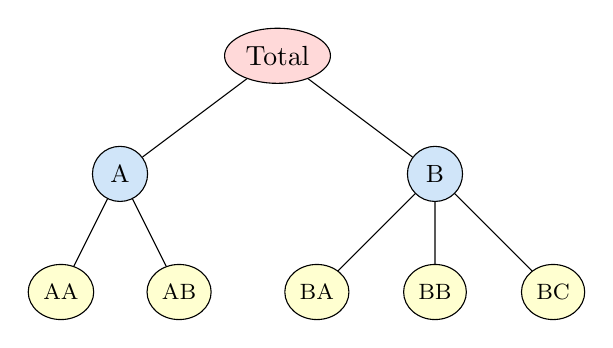
\begin{tikzpicture}
		\tikzstyle{every node}=[ellipse,draw,inner sep=2pt,minimum size=7mm,fill=red!15] %158,202,225
		\tikzstyle[level distance=.1cm]
		\tikzstyle[sibling distance=.1cm]
		%\tikzstyle{level 3}=[sibling distance=6.2mm,font=\tiny]
		\tikzstyle{level 1}=[sibling distance=40mm, font=\small, set style={{every node}+=[fill=hfill_blue]}]
		\tikzstyle{level 2}=[sibling distance=15mm, font=\footnotesize, set style={{every node}+=[fill=hfill_yellow]}]
		\node{Total}%[edge from parent fork down]
		child {node {A}
				child {node {AA}}
				child {node {AB}}
			}
		child {node {B}
				child {node {BA}}
				child {node {BB}}
				child {node {BC}}
			};
	\end{tikzpicture}
	\caption{A simple two-level hierarchical structure.}
	\label{fig:simple tree}
\end{figure}

Let $\bm{y}_t = (y_{\text{Tot},t},y_{\text{A},t}, y_{\text{B},t},y_{\text{AA},t}, y_{\text{AB},t}, y_{\text{BA},t}, y_{\text{BB},t},y_{\text{BC},t})'$ denote a vector containing observations across all series of the hierarchy at time $t$. Similarly denote as $\bm{b}_t = (y_{\text{AA},t}, y_{\text{AB},t}, y_{\text{BA},t}, y_{\text{BB},t}, y_{\text{BC},t})'$ a vector containing observations only for the bottom-level series. In general, $\bm{y}_t\in \varmathbb{R}^n$ and $\bm{b}_t \in \varmathbb{R}^m$ where $n$ denotes the number of total series in the structure, $m$ the number of series at the bottom level, and $n>m$ always. In the simple example of \autoref{fig:simple tree}, $n=8$ and $m=5$.

Aggregation constraints dictate that $y_{\text{Tot}}=y_{\text{A},t}+y_{\text{B},t}=y_{\text{AA},t}+y_{\text{AB},t}+y_{\text{BA},t}+y_{\text{BB},t}+y_{\text{BC},t}$,~ $y_{\text{A},t}=y_{\text{AA},t}+y_{\text{AB},t}$ and $y_{\text{B}}=y_{\text{BA},t}+y_{\text{BB},t}+y_{\text{BC},t}$. Hence we can write
\begin{equation}\label{eq:summing matrix}
	\bm{y}_t = \bm{Sb}_t,
\end{equation}
where \begin{equation*}
	\bm{S} = \begin{pmatrix}
		1 & 1                            & 1 & 1 & 1 \\
		1 & 1                            & 0 & 0 & 0 \\
		0 & 0                            & 1 & 1 & 1 \\
		  & \multicolumn{3}{c}{\bm{I}_5} &
	\end{pmatrix}
\end{equation*}
is an $n\times m$ matrix referred to as the \textit{summing matrix} and $\bm{I}_m$ is an $m$-dimensional identity matrix. $\bm{S}$ reflects the linear aggregation constraints and in particular how the bottom-level series aggregate to levels above. Thus, columns of $\bm{S}$ span the linear subspace of $\varmathbb{R}^n$ for which the aggregation constraints hold. We refer to this as the \textit{coherent subspace} and denote it by $\mathfrak{s}$. Notice that pre-multiplying a vector in $\varmathbb{R}^m$ by $\bm{S}$ will result in an $n$-dimensional vector that lies in $\mathfrak{s}$.

\begin{property}
	A hierarchical time series has observations that are \textit{coherent}, i.e., $\bm{y}_{t} \in \mathfrak{s}$ for all $t$. We use the term coherent to describe not just $\bm{y}_t$ but any vector in $\mathfrak{s}$.
	\label{prop:coherence}
\end{property}

Structures similar to the one shown in \autoref{fig:simple tree} can be found in macroeconomics. For instance, in \autoref{sec:data} we consider two alternative hierarchical structures for the case of GDP and its components. However, while this motivating example involves aggregation constraints, the mathematical framework we use can be applied for any general linear constraints, examples of which are ubiquitous in macroeconomics. For instance, the trade balance is computed as exports minus imports, while the consumer price index is computed as a weighted average of sub-indices, which are in turn weighted averages of sub-sub-indices, and so on. These structures can also be captured by an appropriately designed $\bm{S}$ matrix.

An important alternative aggregation structure, also commonly found in macroeconomics, is one for which the most aggregate series is disaggregated by attributes of interest that are crossed, as distinct to nested which is the case for hierarchical time series. For example, industrial production may be disaggregated along the lines of geography or sector or both. We refer to this as a \textit{grouped} structure. \autoref{fig:simple grouped tree} shows a simple example of such a structure. The Total series disaggregates into $y_{\text{A},t}$ and $y_{\text{B},t}$, but also into $y_{\text{X},t}$ and $y_{\text{Y},t}$, at level 1, and then into the bottom-level series, $\bm{b}_t=(y_{\text{AX}}, y_{\text{AY}}, y_{\text{BX}}, y_{\text{BY}})'$. Hence, in contrast to hierarchical structures, grouped time series do not naturally disaggregate in a unique manner.

\begin{figure}[!hbt]\sidecaption\centering
	\tikzstyle{every node}=[inner sep=2pt,minimum size=7mm]
	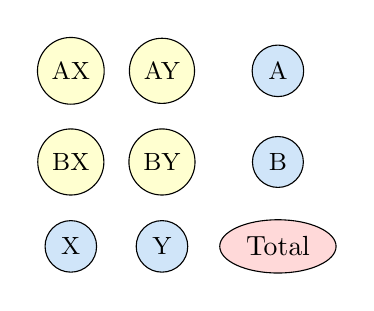
\begin{tikzpicture}
		\matrix[ampersand replacement=\&,column sep=0.3cm] {
			\node[circle,draw,fill=hfill_yellow, font=\small,distance=1cm] {AX};~ \&
			\node[circle,draw,fill=hfill_yellow,font=\small] {AY};~ \&
			\node[circle,draw,fill=hfill_blue, font=\small] {A}; \\[0.3cm]
			\node[circle,draw,fill=hfill_yellow, font=\small] {BX};~ \&
			\node[circle,draw,fill=hfill_yellow, font=\small] {BY};~ \&
			\node[circle,draw,fill=hfill_blue, font=\small] {B}; \\[0.3cm]
			\node[circle,draw,fill=hfill_blue, font=\small] {X};~ \&
			\node[circle,draw,fill=hfill_blue, font=\small] {Y};~ \&
			\node[ellipse,draw,fill=red!15] {Total}; \\
		};
	\end{tikzpicture}
	\caption{A simple two-level grouped structure.}
	\label{fig:simple grouped tree}
\end{figure}

An important implementation of aggregation structures are \textit{temporal hierarchies} introduced by \citet{AthEtAl2017}. In this case the aggregation structure spans the time dimension and dictates how higher frequency data (e.g., monthly) are aggregated to lower frequencies (e.g.\ quarterly, annual). There is a vast literature that studies the effects of temporal aggregation, going back to the seminal work of \citet{ZelMon1971, AmeWu1972, Tia1972, Bre1973} and others, including \citet{Hot1993, HotCar1993, Mar1999, SilEtAl2008}. The main aim of this work is to find the single best level of aggregation for modelling and forecasting time series. In this literature, the analyses, results (whether theoretical or empirical) and inferences, are extremely heterogeneous, making it very challenging to reach a consensus or to draw firm conclusions. For example, \citet{RosSea1995} who study the effect of aggregation on several key macroeconomic variables state:
\begin{quote}
``Quarterly data do not seem to suffer badly from temporal aggregation distortion, nor are they subject to the construction problems affecting monthly data. They therefore may be the optimal data for econometric analysis.''
\end{quote}
A similar conclusion is reached by \citet{NijPal1990}. \citet{SilEtAl2008} consider forecasting French cash state deficit and provide empirical evidence of forecast accuracy gains from forecasting with the aggregate model rather than aggregating forecasts from the disaggregate model.

The vast majority of this literature concentrates on a single level of temporal aggregation \citep[although there are some notable exceptions such as][]{AndEtAl2011,KouEtAl2014}. \citet{AthEtAl2017} show that considering multiple levels of aggregation via temporal hierarchies and implementing forecast reconciliation approaches rather than single level approaches results in substantial gains in forecast accuracy across all levels of temporal aggregation.

\section{Point forecasting}\label{sec:point forecasting}

A requirement when forecasting hierarchical time series is that the forecasts adhere to the same aggregation constraints as the observed data; i.e., they are coherent.

\begin{definition}\label{def:coherence}
	A set of $h$-step-ahead forecasts $\tilde{\bm{y}}_{T+h|T}$, stacked in the same order as $\bm{y}_{t}$ and generated using information up to and including time $T$, are said to be \textit{coherent} if $\tilde{\bm{y}}_{T+h|T} \in \mathfrak{s}$.
\end{definition}

Hence, coherent forecasts of lower level series aggregate to their corresponding upper level series and vice versa.

\begin{figure}[!b]
	\centering
	\vspace{-0.9cm}
	\small
	\resizebox{\linewidth}{!}{
		% Created by tikzDevice version 0.12 on 2019-01-23 11:08:38
% !TEX encoding = UTF-8 Unicode
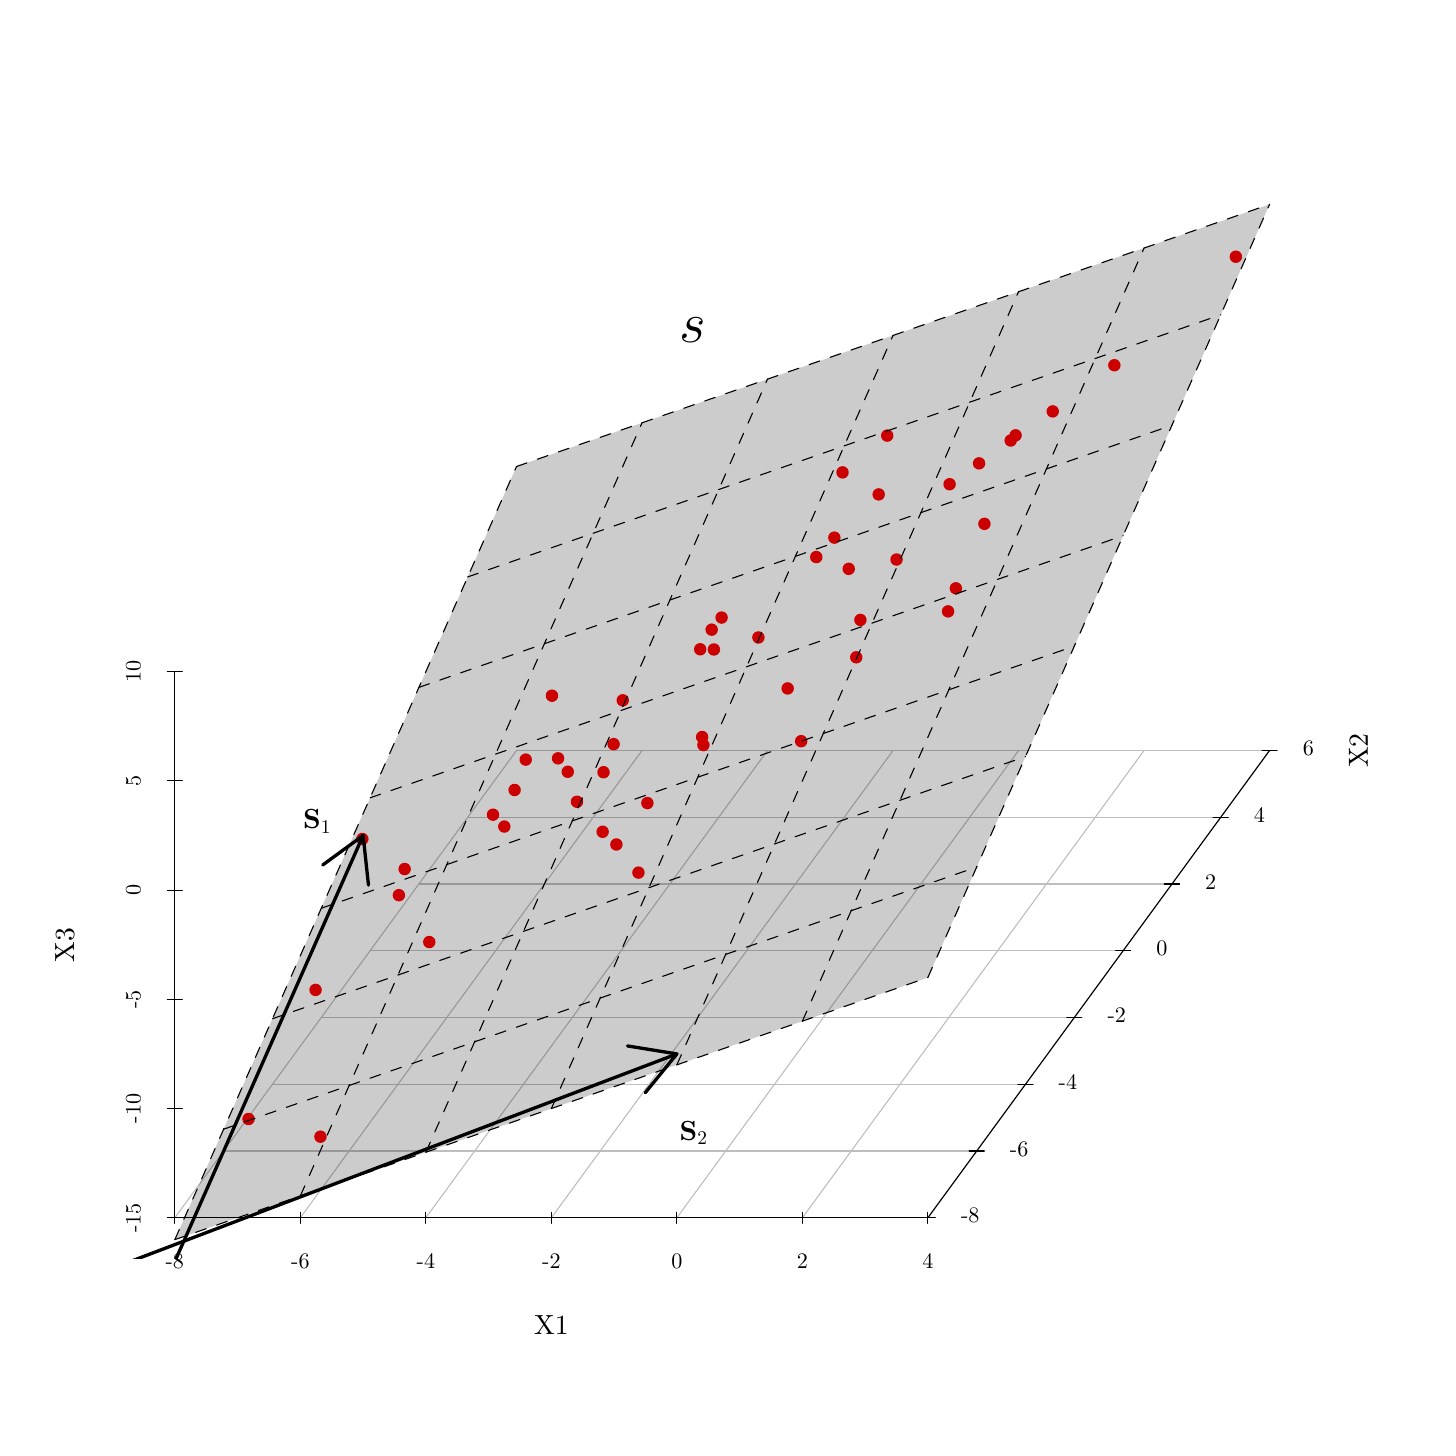
\begin{tikzpicture}[x=1pt,y=1pt]
\definecolor{fillColor}{RGB}{255,255,255}
\path[use as bounding box,fill=fillColor,fill opacity=0.00] (0,0) rectangle (505.89,505.89);
\begin{scope}
\path[clip] ( 37.20, 61.20) rectangle (468.69,456.69);
\definecolor{drawColor}{RGB}{190,190,190}

\path[draw=drawColor,line width= 0.4pt,line join=round,line cap=round] ( 53.18, 75.85) -- (176.64,244.69);

\path[draw=drawColor,line width= 0.4pt,line join=round,line cap=round] ( 98.53, 75.85) -- (221.99,244.69);

\path[draw=drawColor,line width= 0.4pt,line join=round,line cap=round] (143.88, 75.85) -- (267.34,244.69);

\path[draw=drawColor,line width= 0.4pt,line join=round,line cap=round] (189.24, 75.85) -- (312.69,244.69);

\path[draw=drawColor,line width= 0.4pt,line join=round,line cap=round] (234.59, 75.85) -- (358.05,244.69);

\path[draw=drawColor,line width= 0.4pt,line join=round,line cap=round] (279.94, 75.85) -- (403.40,244.69);

\path[draw=drawColor,line width= 0.4pt,line join=round,line cap=round] (325.29, 75.85) -- (448.75,244.69);

\path[draw=drawColor,line width= 0.4pt,line join=round,line cap=round] ( 53.18, 75.85) -- (325.29, 75.85);

\path[draw=drawColor,line width= 0.4pt,line join=round,line cap=round] ( 70.82, 99.97) -- (342.93, 99.97);

\path[draw=drawColor,line width= 0.4pt,line join=round,line cap=round] ( 88.45,124.09) -- (360.57,124.09);

\path[draw=drawColor,line width= 0.4pt,line join=round,line cap=round] (106.09,148.21) -- (378.20,148.21);

\path[draw=drawColor,line width= 0.4pt,line join=round,line cap=round] (123.73,172.33) -- (395.84,172.33);

\path[draw=drawColor,line width= 0.4pt,line join=round,line cap=round] (141.37,196.45) -- (413.48,196.45);

\path[draw=drawColor,line width= 0.4pt,line join=round,line cap=round] (159.00,220.57) -- (431.11,220.57);

\path[draw=drawColor,line width= 0.4pt,line join=round,line cap=round] (176.64,244.69) -- (448.75,244.69);
\definecolor{drawColor}{RGB}{0,0,0}

\path[draw=drawColor,line width= 0.4pt,line join=round,line cap=round] (322.57, 75.85) -- (328.01, 75.85);

\path[draw=drawColor,line width= 0.4pt,line join=round,line cap=round] (340.21, 99.97) -- (345.65, 99.97);

\path[draw=drawColor,line width= 0.4pt,line join=round,line cap=round] (357.84,124.09) -- (363.29,124.09);

\path[draw=drawColor,line width= 0.4pt,line join=round,line cap=round] (375.48,148.21) -- (380.92,148.21);

\path[draw=drawColor,line width= 0.4pt,line join=round,line cap=round] (393.12,172.33) -- (398.56,172.33);

\path[draw=drawColor,line width= 0.4pt,line join=round,line cap=round] (410.75,196.45) -- (416.20,196.45);

\path[draw=drawColor,line width= 0.4pt,line join=round,line cap=round] (428.39,220.57) -- (433.83,220.57);

\path[draw=drawColor,line width= 0.4pt,line join=round,line cap=round] (446.03,244.69) -- (451.47,244.69);

\path[draw=drawColor,line width= 0.4pt,line join=round,line cap=round] ( 53.18, 73.87) -- ( 53.18, 77.82);

\path[draw=drawColor,line width= 0.4pt,line join=round,line cap=round] ( 98.53, 73.87) -- ( 98.53, 77.82);

\path[draw=drawColor,line width= 0.4pt,line join=round,line cap=round] (143.88, 73.87) -- (143.88, 77.82);

\path[draw=drawColor,line width= 0.4pt,line join=round,line cap=round] (189.24, 73.87) -- (189.24, 77.82);

\path[draw=drawColor,line width= 0.4pt,line join=round,line cap=round] (234.59, 73.87) -- (234.59, 77.82);

\path[draw=drawColor,line width= 0.4pt,line join=round,line cap=round] (279.94, 73.87) -- (279.94, 77.82);

\path[draw=drawColor,line width= 0.4pt,line join=round,line cap=round] (325.29, 73.87) -- (325.29, 77.82);

\path[draw=drawColor,line width= 0.4pt,line join=round,line cap=round] ( 50.46, 75.85) -- ( 55.90, 75.85);

\path[draw=drawColor,line width= 0.4pt,line join=round,line cap=round] ( 50.46,115.32) -- ( 55.90,115.32);

\path[draw=drawColor,line width= 0.4pt,line join=round,line cap=round] ( 50.46,154.79) -- ( 55.90,154.79);

\path[draw=drawColor,line width= 0.4pt,line join=round,line cap=round] ( 50.46,194.26) -- ( 55.90,194.26);

\path[draw=drawColor,line width= 0.4pt,line join=round,line cap=round] ( 50.46,233.73) -- ( 55.90,233.73);

\path[draw=drawColor,line width= 0.4pt,line join=round,line cap=round] ( 50.46,273.20) -- ( 55.90,273.20);
\end{scope}
\begin{scope}
\path[clip] (  0.00,  0.00) rectangle (505.89,505.89);
\definecolor{drawColor}{RGB}{0,0,0}

\node[text=drawColor,anchor=base,inner sep=0pt, outer sep=0pt, scale=  0.80] at ( 53.18, 57.60) {-8};

\node[text=drawColor,anchor=base,inner sep=0pt, outer sep=0pt, scale=  0.80] at ( 98.53, 57.60) {-6};

\node[text=drawColor,anchor=base,inner sep=0pt, outer sep=0pt, scale=  0.80] at (143.88, 57.60) {-4};

\node[text=drawColor,anchor=base,inner sep=0pt, outer sep=0pt, scale=  0.80] at (189.24, 57.60) {-2};

\node[text=drawColor,anchor=base,inner sep=0pt, outer sep=0pt, scale=  0.80] at (234.59, 57.60) { 0};

\node[text=drawColor,anchor=base,inner sep=0pt, outer sep=0pt, scale=  0.80] at (279.94, 57.60) { 2};

\node[text=drawColor,anchor=base,inner sep=0pt, outer sep=0pt, scale=  0.80] at (325.29, 57.60) { 4};

\node[text=drawColor,rotate= 90.00,anchor=base,inner sep=0pt, outer sep=0pt, scale=  0.80] at ( 40.80, 75.85) {-15};

\node[text=drawColor,rotate= 90.00,anchor=base,inner sep=0pt, outer sep=0pt, scale=  0.80] at ( 40.80,115.32) {-10};

\node[text=drawColor,rotate= 90.00,anchor=base,inner sep=0pt, outer sep=0pt, scale=  0.80] at ( 40.80,154.79) { -5};

\node[text=drawColor,rotate= 90.00,anchor=base,inner sep=0pt, outer sep=0pt, scale=  0.80] at ( 40.80,194.26) {  0};

\node[text=drawColor,rotate= 90.00,anchor=base,inner sep=0pt, outer sep=0pt, scale=  0.80] at ( 40.80,233.73) {  5};

\node[text=drawColor,rotate= 90.00,anchor=base,inner sep=0pt, outer sep=0pt, scale=  0.80] at ( 40.80,273.20) { 10};
\end{scope}
\begin{scope}
\path[clip] ( 37.20, 61.20) rectangle (468.69,456.69);
\definecolor{drawColor}{RGB}{0,0,0}

\node[text=drawColor,anchor=base west,inner sep=0pt, outer sep=0pt, scale=  0.80] at (337.29, 74.01) {-8};

\node[text=drawColor,anchor=base west,inner sep=0pt, outer sep=0pt, scale=  0.80] at (354.93, 98.13) {-6};

\node[text=drawColor,anchor=base west,inner sep=0pt, outer sep=0pt, scale=  0.80] at (372.57,122.25) {-4};

\node[text=drawColor,anchor=base west,inner sep=0pt, outer sep=0pt, scale=  0.80] at (390.20,146.37) {-2};

\node[text=drawColor,anchor=base west,inner sep=0pt, outer sep=0pt, scale=  0.80] at (407.84,170.49) { 0};

\node[text=drawColor,anchor=base west,inner sep=0pt, outer sep=0pt, scale=  0.80] at (425.48,194.61) { 2};

\node[text=drawColor,anchor=base west,inner sep=0pt, outer sep=0pt, scale=  0.80] at (443.11,218.73) { 4};

\node[text=drawColor,anchor=base west,inner sep=0pt, outer sep=0pt, scale=  0.80] at (460.75,242.86) { 6};

\path[draw=drawColor,line width= 0.4pt,line join=round,line cap=round] ( 53.18, 75.85) --
	(325.29, 75.85);
\end{scope}
\begin{scope}
\path[clip] (  0.00,  0.00) rectangle (505.89,505.89);
\definecolor{drawColor}{RGB}{0,0,0}

\node[text=drawColor,anchor=base,inner sep=0pt, outer sep=0pt, scale=  1.00] at (189.24, 33.60) {X1};
\end{scope}
\begin{scope}
\path[clip] ( 37.20, 61.20) rectangle (468.69,456.69);
\definecolor{drawColor}{RGB}{0,0,0}

\path[draw=drawColor,line width= 0.4pt,line join=round,line cap=round] (325.29, 75.85) --
	(448.75,244.69);
\end{scope}
\begin{scope}
\path[clip] (  0.00,  0.00) rectangle (505.89,505.89);
\definecolor{drawColor}{RGB}{0,0,0}

\node[text=drawColor,rotate= 90.00,anchor=base,inner sep=0pt, outer sep=0pt, scale=  1.00] at (484.29,244.69) {X2};
\end{scope}
\begin{scope}
\path[clip] ( 37.20, 61.20) rectangle (468.69,456.69);
\definecolor{drawColor}{RGB}{0,0,0}

\path[draw=drawColor,line width= 0.4pt,line join=round,line cap=round] ( 53.18, 75.85) --
	( 53.18,273.20);
\end{scope}
\begin{scope}
\path[clip] (  0.00,  0.00) rectangle (505.89,505.89);
\definecolor{drawColor}{RGB}{0,0,0}

\node[text=drawColor,rotate= 90.00,anchor=base,inner sep=0pt, outer sep=0pt, scale=  1.00] at ( 16.80,174.52) {X3};
\end{scope}
\begin{scope}
\path[clip] ( 37.20, 61.20) rectangle (468.69,456.69);
\definecolor{fillColor}{RGB}{255,0,0}

\path[fill=fillColor] (436.57,423.12) circle (  2.25);

\path[fill=fillColor] (310.59,358.48) circle (  2.25);

\path[fill=fillColor] (392.67,383.91) circle (  2.25);

\path[fill=fillColor] (294.45,345.19) circle (  2.25);

\path[fill=fillColor] (370.39,367.23) circle (  2.25);

\path[fill=fillColor] (356.98,358.58) circle (  2.25);

\path[fill=fillColor] (355.21,356.71) circle (  2.25);

\path[fill=fillColor] (307.51,337.23) circle (  2.25);

\path[fill=fillColor] (343.78,348.45) circle (  2.25);

\path[fill=fillColor] (333.13,340.91) circle (  2.25);

\path[fill=fillColor] (291.49,321.61) circle (  2.25);

\path[fill=fillColor] (284.96,314.59) circle (  2.25);

\path[fill=fillColor] (296.68,310.34) circle (  2.25);

\path[fill=fillColor] (345.72,326.59) circle (  2.25);

\path[fill=fillColor] (250.75,292.73) circle (  2.25);

\path[fill=fillColor] (313.96,313.70) circle (  2.25);

\path[fill=fillColor] (247.16,288.36) circle (  2.25);

\path[fill=fillColor] (189.45,264.50) circle (  2.25);

\path[fill=fillColor] (243.02,281.27) circle (  2.25);

\path[fill=fillColor] (247.96,281.19) circle (  2.25);

\path[fill=fillColor] (264.05,285.54) circle (  2.25);

\path[fill=fillColor] (215.03,262.83) circle (  2.25);

\path[fill=fillColor] (300.90,291.88) circle (  2.25);

\path[fill=fillColor] (335.40,303.30) circle (  2.25);

\path[fill=fillColor] (332.58,294.96) circle (  2.25);

\path[fill=fillColor] (179.97,241.40) circle (  2.25);

\path[fill=fillColor] (191.66,241.87) circle (  2.25);

\path[fill=fillColor] (299.40,278.37) circle (  2.25);

\path[fill=fillColor] (211.73,246.99) circle (  2.25);

\path[fill=fillColor] (274.62,267.12) circle (  2.25);

\path[fill=fillColor] (120.93,212.71) circle (  2.25);

\path[fill=fillColor] (175.95,230.42) circle (  2.25);

\path[fill=fillColor] (195.16,237.01) circle (  2.25);

\path[fill=fillColor] (243.71,249.56) circle (  2.25);

\path[fill=fillColor] (208.09,236.84) circle (  2.25);

\path[fill=fillColor] (168.15,221.49) circle (  2.25);

\path[fill=fillColor] (244.17,246.66) circle (  2.25);

\path[fill=fillColor] (172.23,217.21) circle (  2.25);

\path[fill=fillColor] (198.50,226.18) circle (  2.25);

\path[fill=fillColor] (136.21,201.87) circle (  2.25);

\path[fill=fillColor] (279.49,248.06) circle (  2.25);

\path[fill=fillColor] (223.93,225.70) circle (  2.25);

\path[fill=fillColor] (134.14,192.41) circle (  2.25);

\path[fill=fillColor] (207.76,215.33) circle (  2.25);

\path[fill=fillColor] (212.73,210.74) circle (  2.25);

\path[fill=fillColor] (145.12,175.48) circle (  2.25);

\path[fill=fillColor] (220.70,200.57) circle (  2.25);

\path[fill=fillColor] (104.03,158.19) circle (  2.25);

\path[fill=fillColor] ( 79.81,111.54) circle (  2.25);

\path[fill=fillColor] (105.79,105.14) circle (  2.25);
\definecolor{fillColor}{RGB}{0,0,0}

\path[fill=fillColor,fill opacity=0.20] ( 53.18, 67.95) --
	(176.64,347.31) --
	(448.75,442.04) --
	(325.29,162.68) --
	cycle;
\definecolor{drawColor}{RGB}{0,0,0}

\path[draw=drawColor,line width= 0.4pt,dash pattern=on 4pt off 4pt ,line join=round,line cap=round] ( 53.18, 67.95) -- (176.64,347.31);

\path[draw=drawColor,line width= 0.4pt,dash pattern=on 4pt off 4pt ,line join=round,line cap=round] ( 98.53, 83.74) -- (221.99,363.10);

\path[draw=drawColor,line width= 0.4pt,dash pattern=on 4pt off 4pt ,line join=round,line cap=round] (143.88, 99.53) -- (267.34,378.89);

\path[draw=drawColor,line width= 0.4pt,dash pattern=on 4pt off 4pt ,line join=round,line cap=round] (189.24,115.32) -- (312.69,394.68);

\path[draw=drawColor,line width= 0.4pt,dash pattern=on 4pt off 4pt ,line join=round,line cap=round] (234.59,131.11) -- (358.05,410.47);

\path[draw=drawColor,line width= 0.4pt,dash pattern=on 4pt off 4pt ,line join=round,line cap=round] (279.94,146.89) -- (403.40,426.25);

\path[draw=drawColor,line width= 0.4pt,dash pattern=on 4pt off 4pt ,line join=round,line cap=round] (325.29,162.68) -- (448.75,442.04);

\path[draw=drawColor,line width= 0.4pt,dash pattern=on 4pt off 4pt ,line join=round,line cap=round] ( 53.18, 67.95) -- (325.29,162.68);

\path[draw=drawColor,line width= 0.4pt,dash pattern=on 4pt off 4pt ,line join=round,line cap=round] ( 70.82,107.86) -- (342.93,202.59);

\path[draw=drawColor,line width= 0.4pt,dash pattern=on 4pt off 4pt ,line join=round,line cap=round] ( 88.45,147.77) -- (360.57,242.50);

\path[draw=drawColor,line width= 0.4pt,dash pattern=on 4pt off 4pt ,line join=round,line cap=round] (106.09,187.68) -- (378.20,282.41);

\path[draw=drawColor,line width= 0.4pt,dash pattern=on 4pt off 4pt ,line join=round,line cap=round] (123.73,227.59) -- (395.84,322.32);

\path[draw=drawColor,line width= 0.4pt,dash pattern=on 4pt off 4pt ,line join=round,line cap=round] (141.37,267.50) -- (413.48,362.22);

\path[draw=drawColor,line width= 0.4pt,dash pattern=on 4pt off 4pt ,line join=round,line cap=round] (159.00,307.41) -- (431.11,402.13);

\path[draw=drawColor,line width= 0.4pt,dash pattern=on 4pt off 4pt ,line join=round,line cap=round] (176.64,347.31) -- (448.75,442.04);

\path[draw=drawColor,line width= 1.2pt,line join=round,line cap=round] ( 26.64,  0.00) -- (121.21,213.99);

\path[draw=drawColor,line width= 1.2pt,line join=round,line cap=round] (123.15,196.03) --
	(121.21,213.99) --
	(106.62,203.33);

\path[draw=drawColor,line width= 1.2pt,line join=round,line cap=round] (  0.00, 45.96) -- (234.59,135.05);

\path[draw=drawColor,line width= 1.2pt,line join=round,line cap=round] (223.17,121.05) --
	(234.59,135.05) --
	(216.75,137.94);

\node[text=drawColor,anchor=base west,inner sep=0pt, outer sep=0pt, scale=  1.00] at ( 99.52,216.34) {\bfseries S};

\node[text=drawColor,anchor=base west,inner sep=0pt, outer sep=0pt, scale=  0.70] at (105.91,214.83) {1};

\node[text=drawColor,anchor=base west,inner sep=0pt, outer sep=0pt, scale=  1.00] at (235.58,103.85) {\bfseries S};

\node[text=drawColor,anchor=base west,inner sep=0pt, outer sep=0pt, scale=  0.70] at (241.96,102.34) {2};

\node[text=drawColor,anchor=base west,inner sep=0pt, outer sep=0pt, scale=  1.00] at (235.51,392.30) {{\huge $\mathfrak{s}$}};
\end{scope}
\end{tikzpicture}

	}
	\caption{Representation of a coherent subspace in a three dimensional hierarchy where $y_{\text{Tot}} = y_{\text{A}} + y_{\text{B}}$. The coherent subspace is depicted as a gray two dimensional plane labelled $\mathfrak{s}$. Note that the columns of $\vec{s}_1 = (1,1,0)'$ and $\vec{s}_2 = (1, 0, 1)'$ form a basis for $\mathfrak{s}$. The red points lying on $\mathfrak{s}$ can be either realisations or coherent forecasts.}\label{fig:Schematic-3D}
\end{figure}

Let us consider the smallest possible hierarchy with two bottom-level series, depicted in \autoref{fig:Schematic-3D}, where $y_{\text{Tot}} = y_{\text{A}} + y_{\text{B}}$. While base forecasts could lie anywhere in $\varmathbb{R}^3$, the realisations and coherent forecasts lie in a two dimensional subspace $\mathfrak{s}\subset \varmathbb{R}^3$.

\subsection{Single-level approaches}\label{sec:single level approaches}
A common theme across all traditional approaches for forecasting hierarchical time series is that a single-level of aggregation is first selected and forecasts for that level are generated. These are then linearly combined to generate a set of coherent forecasts the rest of the structure.

\subsubsection{Bottom-up}

In the \textit{bottom-up} approach, forecasts for the most disaggregate level are first generated. These are then aggregated to obtain forecasts for all other series of the hierarchy \citep{dunn1976}. In general, this consists of first generating $\hat{\bm{b}}_{T+h|T} \in \varmathbb{R}^m$, a set of $h$-step-ahead forecasts for the bottom-level series. For the simple hierarchical structure of \autoref{fig:simple tree}, $\hat{\bm{b}}_{T+h|T} = (\hat{{y}}_{\text{AA},T+h|T}, \hat{{y}}_{\text{AB},T+h|T}, \hat{{y}}_{\text{BA},T+h|T}, \hat{{y}}_{\text{BB},T+h|T},\hat{{y}}_{\text{BC},T+h|T}),$ where $\hat{{y}}_{i,T+h|T}$ is the $h$-step-ahead forecast of the series corresponding to node $i$. A set of coherent forecasts for the whole hierarchy is then given by
\begin{equation*}\label{eq:BU}
	\tilde{\bm{y}}^{\text{BU}}_{T+h|T}=\bm{S\hat{\bm{b}}}_{T+h|T}.
\end{equation*}
Generating bottom-up forecasts has the advantage of no information being lost due to aggregation. However, bottom-level data can potentially be highly volatile or very noisy and therefore challenging to forecast.

\subsubsection{Top-down}

In contrast, \textit{top-down} approaches involve first generating forecasts for the most aggregate level and then disaggregating these down the hierarchy. In general, coherent forecasts generated from top-down approaches are given by
\begin{equation*}
	\tilde{\bm{y}}^{\text{TD}}_{T+h|T}=\bm{S}\bm{p}\hat{y}_{\text{Tot}, T+h|T},
\end{equation*}
where $\bm{p} = (p_1,\dots,p_m)'$ is an $m$-dimensional vector consisting of a set of proportions which disaggregate the top-level forecast $\hat{y}_{\text{Tot}, T+h|T}$ to forecasts for the bottom-level series; hence $\bm{p}\hat{y}_{\text{Tot}, T+h|T}=\bm{\hat{\bm{b}}}_{T+h|T}$. These are then aggregated by the summing matrix $\bm{S}$.

Traditionally, proportions have been calculated based on the observed historical data. \citet{gross1990} present and evaluate twenty-one alternative approaches. The most convenient attribute of these approaches is their simplicity. Generating a set of coherent forecasts involves only modelling and generating forecasts for the most aggregate top-level series. In general, such top-down approaches seem to produce quite reliable forecasts for the aggregate levels and they are useful with low count data. However, a significant disadvantage is the loss of information due to aggregation. A limitation of such top-down approaches is that characteristics of lower level series cannot be captured. To overcome this, \citet{AthEtAl2009} introduced a new top-down approach which disaggregates the top-level based on proportions of forecasts rather than the historical data and showed that this method outperforms the conventional top-down approaches. However, a limitation of all top-down approaches is that they introduce bias to the forecasts even when the top-level forecast itself is unbiased. We discuss this in detail in \autoref{sec:reconciliation approaches}.

\subsubsection{Middle-out}

A compromise between bottom-up and top-down approaches is the middle-out approach. It entails first forecasting the series of a selected middle-level. For series above the middle-level, coherent forecasts are generated using the bottom-up approach by aggregating the middle-level forecasts. For series below the middle level, coherent forecasts are generated using a top-down approach by disaggregating the middle-level forecasts. Since the middle-out approach involves generating top-down forecasts, it also introduces bias to the forecasts.

\subsection{Point forecast reconciliation}\label{sec:reconciliation approaches}

All approaches discussed so far are limited to only using information from a single-level of aggregation. Furthermore, these ignore any correlations across levels of a hierarchy. An alternative framework that overcomes these limitations is one that involves forecast \textit{reconciliation}. In a first step. forecasts for all the series across all levels of the hierarchy are computed, ignoring any aggregation constraints. We refer to these as \textit{base} forecasts and denote them by $\hat{\bm{y}}_{T+h|T}$. In general, base forecasts will not be coherent, unless a very simple method has been used to compute them such as for \naive forecasts. In this case, forecasts are simply equal to a previous realisation of the data and they inherit the property of coherence.

The second step is an adjustment that reconciles base forecasts so that they become coherent. In general, this is achieved by mapping the base forecasts $\hat{\bm{y}}_{T+h|T}$ onto the coherent subspace $\mathfrak{s}$ via a matrix $\bm{S}\bm{G}$, resulting in a set of coherent forecasts $\tilde{\bm{y}}_{T+h|T}$. Specifically,
\begin{equation}\label{eq:recon}
	\tilde{\bm{y}}_{T+h|T}=\bm{S}\bm{G}\hat{\bm{y}}_{T+h|T},
\end{equation}
where $\bm{G}$ is an $m\times n$ matrix that maps $\hat{\bm{y}}_{T+h|T}$ to $\varmathbb{R}^m$, producing new forecasts for the bottom level, which are in turn mapped to the coherent subspace by the summing matrix $\bm{S}$. We restrict our attention to projections on $\mathfrak{s}$ in which case $\bm{S}\bm{G}\bm{S}=\bm{S}$. This ensures that unbiasedness is preserved, i.e., for a set of unbiased base forecasts reconciled forecasts will also be unbiased.

Note that all single-level approaches discussed so far can also be represented by \eqref{eq:recon} using appropriately designed $\bm{G}$ matrices, however not all of these will be projections. For example for the bottom-up approach, $\bm{G}=\begin{pmatrix}
		\bm{0}_{(m \times n-m)} & \bm{I}_m
	\end{pmatrix}$ in which case $\bm{S}\bm{G}\bm{S}=\bm{S}$. For any top-down approach
$\bm{G}=\begin{pmatrix}
		\bm{p} & \bm{0}_{(m \times n-1)}
	\end{pmatrix}$, for which $\bm{S}\bm{G}\bm{S}\ne\bm{S}$.

\subsubsection{Optimal MinT reconciliation}

\citet{WicEtAl2019} build a unifying framework for much of the previous literature on forecast reconciliation. We present here a detailed outline of this approach and in turn relate it to previous significant contributions in forecast reconciliation.

Assume that $\hat{\bm{y}}_{T+h|T}$ is a set of unbiased base forecasts, i.e., $\E_{1:T}(\hat{\bm{y}}_{T+h|T})= \E_{1:T}[\bm{y}_{T+h}\mid\bm{y}_1,\dots,\bm{y}_T]$, the true mean with the expectation taken over the observed sample up to time $T$.
Let
\begin{equation}\label{eq:base errors}
	\hat{\bm{e}}_{T+h|T} = \bm{y}_{T+h|T}-\hat{\bm{y}}_{T+h|T}
\end{equation}
denote a set of base forecast errors with Var$(\hat{\bm{e}}_{T+h|T})=\bm{W}_h$, and
\begin{equation*}
	\tilde{\bm{e}}_{T+h|T} = \bm{y}_{T+h|T}-\tilde{\bm{y}}_{T+h|T}
\end{equation*} denote a set of coherent forecast errors. Lemma 1 in \citet{WicEtAl2019} shows that for any matrix $\bm{G}$ such that $\bm{S}\bm{G}\bm{S}=\bm{S}$, $\text{Var}(\tilde{\bm{e}}_{T+h|T})=\bm{S}\bm{G}\bm{W}_h\bm{S}'\bm{G}'
$. Furthermore Theorem 1 shows that
\begin{equation} \label{eq:MinT}
	\bm{G} = (\bm{S}'{\bm{W}}^{-1}_h\bm{S})^{-1}\bm{S}'{\bm{W}}^{-1}_h
\end{equation}
is the unique solution that minimises the trace of $\bm{S}\bm{G}\bm{W}_h\bm{S}'\bm{G}'$ subject to $\bm{S}\bm{G}\bm{S}=\bm{S}$. MinT is optimal in the sense that given a set of unbiased base forecasts, it returns a set of best linear unbiased reconciled forecasts, using as $\bm{G}$ the unique solution that minimises the trace (hence MinT) of the variance of the forecast error of the reconciled forecasts.

A significant advantage of the MinT reconciliation solution is that it is the first to incorporate the full correlation structure of the hierarchy via $\bm{W}_{h}$. However, estimating $\bm{W}_{h}$ is challenging, especially for $h>1$. \citet{WicEtAl2019} present possible alternative estimators for $\bm{W}_{h}$ and show that these lead to different $\bm{G}$ matrices. We summarise these below.

\begin{itemize}\parskip=1.2ex
	\item Set $\bm{W}_{h}=k_h\bm{I}_n$ for all $h$, where $k_{h} > 0$ is a proportionality constant. This simple assumption returns $\bm{G}=(\bm{S}'\bm{S})^{-1}\bm{S}'$ so that the base forecasts are orthogonally projected onto the coherent subspace $\mathfrak{s}$ minimising the Euclidean distance between $\hat{\bm{y}}_{T+h|T}$ and $\tilde{\bm{y}}_{T+h|T}$. \citet{HynEtAl2011} come to same solution, however from the perspective of the following regression model
  \begin{equation*}
    \hat{\bm{y}}_{T+h|T} = \bm{S}\bm{\beta}_{T+h|T} + \bm{\varepsilon}_{T+h|T},
  \end{equation*}
  where $\bm{\beta}_{T+h|T}=\E[\bm{b}_{T+h}\mid\bm{b}_1,\dots,\bm{b}_T]$ is the unknown conditional mean of the bottom-level series and $\bm{\varepsilon}_{T+h|T}$ is the coherence or reconciliation error with mean zero and variance $\bm{V}$. The OLS solution leads to the same projection matrix $\bm{S}(\bm{S}'\bm{S})^{-1}\bm{S}'$, and due to this interpretation we continue to refer to this reconciliation method as OLS\@. A disadvantage of the OLS solution is that the homoscedastic diagonal entries do not account for the scale differences between the levels of the hierarchy due to aggregation. Furthermore, OLS does not account for the correlations across series.

	\item Set ${\bm{W}}_{h}=k_{h}\text{diag}(\hat{\bm{W}}_{1})$ for all $h$ ($k_{h} > 0$), where
  $$
    \hat{\bm{W}}_{1} = \frac{1}{T}\sum_{T=1}^{T} \hat{\bm{e}}_{t}\hat{\bm{e}}_{t}'
  $$
  is the unbiased sample estimator of the in-sample one-step-ahead base forecast errors as defined in~\eqref{eq:base errors}. Hence this estimator scales the base forecasts using the variance of the in-sample residuals and is therefore described and referred to as a weighted least squares (WLS) estimator applying variance scaling. A similar estimator was proposed by \citet{Hyndman2016}.

  An alternative WLS estimator is proposed by \citet{AthEtAl2017} in the context of temporal hierarchies. Here $\bm{W}_{h}$ is proportional to $\text{diag}(\bm{S}\bm{1})$ where $\bm{1}$ is a unit column vector of dimension $n$. Hence the weights are proportional to the number of bottom-level variables required to form an aggregate. For example, in the hierarchy of \autoref{fig:simple tree}, the weights corresponding to the Total, series A and series B are proportional to 5, 2 and 3 respectively. This weighting scheme depends only on the aggregation structure and is referred to as structural scaling. Its advantage over OLS is that it assumes equivariant forecast errors only at the bottom level of the structure and not across all levels. It is particularly useful in cases where forecast errors are not available; for example, in cases where the base forecasts are generated by judgemental forecasting.

	\item Set $\bm{W}_{h}=k_{h}\hat{\bm{W}}_{1}$ for all $h$ ($k_{h} > 0$) to be proportional to the unrestricted sample covariance estimator for $h=1$. Although this is relatively simple to obtain and provides a good solution for small hierarchies, it does not provide reliable results as $m$ grows compared to $T$. This is referred to this as the MinT(Sample) estimator.

	\item Set $\bm{W}_{h}=k_{h}\hat{\bm{W}}_{1}^D$ for all $h$ ($k_{h} > 0$), where $\hat{\bm{W}}^{D}_{1} = \lambda_{D} \text{diag}(\hat{\bm{W}}_{1}) + (1 - \lambda_{D})\hat{\bm{W}}_{1}$ is a shrinkage estimator with diagonal target and shrinkage intensity parameter
  $$
    \hat{\lambda}_{D} = \frac{\sum_{i \ne j}\hat{\text{Var}}(\hat{r}_{ij})}{\sum_{i \ne j}\hat{r}_{ij}^2},
  $$
	where $\hat{r}_{ij}$ is the $(i,j)$th element of $\hat{\bm{R}}_{1}$, the one-step-ahead sample correlation matrix as proposed by \citet{Schafer2005}. Hence, off-diagonal elements of $\hat{\bm{W}}_1$ are shrunk towards zero while diagonal elements (variances) remain unchanged. This is referred to as the MinT(Shrink) estimator.
\end{itemize}

\section{Hierarchical probabilistic forecasting}\label{sec:probforecasting}

A limitation of point forecasts is that they provide no indication of uncertainty around the forecast. A richer description of forecast uncertainty can be obtained by providing a probabilistic forecast, also commonly referred to as a density forecast. For a review of probabilistic forecasts, and \emph{scoring rules} for evaluating such forecasts, see \citep{Gneiting2014}. In recent years, the use of probabilistic forecasts and their evaluation via scoring rules has become pervasive in macroeconomic forecasting, some notable (but non-exhaustive) examples are \citet{GewAmi2010}, \citet{BilEtAl2013}, \citet{CarEtAl2015} and \citet{ClaRav2015}.

The literature on hierarchical probabilistic forecasting is still an emerging area of interest.  To the best of our knowledge the first attempt to even define coherence in the setting of probabilistic forecasting is provided by \citet{Taieb2017} who define a coherent forecast in terms of a convolution. An equivalent definition due to \citet{GamEtAl2018} defines a coherent probabilistic forecast as a probability measure on the coherent subspace $\mathfrak{s}$. \citet{GamEtAl2018} also generalise the concept of forecast reconciliation to the probabilistic setting.

\begin{definition} Let $\mathcal{A}$ be a subset\footnote{Strictly speaking $\mathcal{A}$ is a Borel set} of $\mathfrak{s}$ and let $\mathcal{B}$ be all points in $\varmathbb{R}^n$ that are mapped onto $\mathcal{A}$ after premultiplication by $\bm{S}\bm{G}$. Letting $\hat{\nu}$ be a base probabilistic forecast for the full hierarchy, the coherent measure $\tilde{\nu}$ reconciles $\hat{\nu}$ if $\tilde{\nu}(\mathcal{A})=\hat{\nu}(\mathcal{B})$ for all $\mathcal{A}$.
\end{definition}

In practice this definition leads to two approaches. For some parametric distributions, for instance the multivariate normal, a reconciled probabilistic forecast can be derived analytically. However, in macroeconomic forecasting, non-standard distributions such as bimodal distributions are often required to take different policy regimes into account. In such cases a non-parametric approach based on bootstrapping in-sample errors proposed \citet{GamEtAl2018} can be used. These scenarios are now covered in detail.

\subsection{Probabilistic forecast reconciliation in the Gaussian framework}\label{sec:probrecgauss}

In the case where the base forecasts are probabilistic forecasts characterised by elliptical distributions, \citet{GamEtAl2018} show that reconciled probabilistic forecasts will also be elliptical. This is particularly straightforward for the Gaussian distribution which is completely characterised by two moments. Letting the base probabilistic forecasts be $\mathscr{N}(\bm{\hat{y}}_{T+h|T}, \hat{\bm{\Sigma}}_{T+h|T})$, then the reconciled probabilistic forecasts will be $\mathscr{N}(\bm{\tilde{y}}_{T+h|T}, \tilde{\bm{\Sigma}}_{T+h|T})$, where
\begin{align}\label{eq:rec mean}
	\bm{\tilde{y}}_{T+h|T} &= \bm{S}\bm{G}\bm{\hat{y}}_{T+h|T} \\
\text{and}\qquad\label{eq:rec var}
	\tilde{\bm{\Sigma}}_{T+h|T} &= \bm{S}\bm{G}\hat{\bm{\Sigma}}_{T+h|T}\bm{G}'\bm{S}'.
\end{align}

There are several options for obtaining the base probabilistic forecasts and in particular the variance covariance matrix $\hat{\bm{\Sigma}}$. One option is to fit multivariate models either level by level or for the hierarchy as a whole leading respectively to a $\hat{\bm \Sigma}$ that is block diagonal or dense. Another option is to fit univariate models for each individual series in which case $\hat{\bm{\Sigma}}$ is a diagonal matrix. A third option that we employ here is to obtain $\hat{\bm{\Sigma}}$ using in-sample forecast errors, in a similar vein to how $\hat{\bm{W}}_{1}$ is estimated in the MinT method. Here the same shrinkage estimator described in \autoref{sec:reconciliation approaches} is used. The reconciled probabilistic forecast will ultimately depend on the choice of $\bm{G}$; the same choices of $\bm{G}$ matrices used in \autoref{sec:point forecasting} can be used.

\subsection{Probabilistic forecast reconciliation in the non-parametric framework}\label{sec:probrecnp}

In many applications, including macroeconomic forecasting, it may not be reasonable to assume Gaussian predictive distributions. Therefore, non-parametric approaches have been widely used for probabilistic forecasts in different disciplines. For example, ensemble forecasting in weather applications \citep{GneRaf2005,Gneiting2014,Gneiting2008}, and bootstrap based approaches \citep{Manzan2008,Vilar2013}. In macroeconomics, \citet{CogEtAl2005} discuss the importance of allowing for skewness in density forecasts and more recently \citet{SmiVah2016} discuss this issue in detail.

Due to these concerns, we employ the bootstrap method proposed by \citet{GamEtAl2018} that does not make parametric assumptions about the predictive distribution. An important result exploited by this method is that applying point forecast reconciliation to the draws from an incoherent base predictive distribution, results in a sample from the reconciled predictive distribution. We summarise this process below:

\begin{enumerate}
	\item Fit univariate models to each series in the hierarchy over a training set from $t=1,\dots,T$.
	\item For each series compute $h$-step-ahead point forecasts, for $h=1,\dots,H$. Collect these into an $n\times H$ matrix $\hat{\bm{Y}}:=(\hat{\bm{y}}_{T+1|T},\dots,\hat{\bm{y}}_{T+H|T})$, where $\hat{\bm{y}}_{T+h|T}$ is an $n$-vector of $h$-step-ahead point forecasts for all series in the hierarchy.
	\item Compute one-step-ahead in-sample forecast errors. Collect these into an $n \times T$ matrix ${\hat{\bm E}}=(\hat{\bm{e}}_1,\hat{\bm{e}}_2,\dots,\hat{\bm{e}}_T)$, where the $n$-vector $\hat{\bm{e}}_t={\bm{y}}_t-\hat{\bm {y}}_{t|t-1}$. Here, $\hat{\bm {y}}_{t|t-1}$ is a vector of forecasts made for time $t$ using information up to and including time $t-1$. These are called in-sample forecasts since while they depend only on past values, information from the entire training sample is used to estimate the parameters for the models on which the forecasts are based.
	\item Block bootstrap from $\hat{\bm{E}}$; that is choose $H$ consecutive columns of $\hat{{\bm E}}$ at random, repeating this process $B$ times. Denote the $n\times H$ matrix obtained at iteration $b$ as $\hat{{\bm E}}^b$ for $b=1,\dots,B$.
	\item For all $b$, compute $\hat{\bm\Upsilon}^b:=\hat{\bm{Y}}+\hat{\bm{E}}^b$. Each row of $\hat{\bm \Upsilon}^b$ is a sample path of $h$ forecasts for a single series. Each column of $\hat{\bm \Upsilon}^b$ is a realisation from the joint predictive distribution at a particular horizon.
	\item For each $b=1,\dots,B$, select the $h$th column of $\hat{\bm \Upsilon}^b$ and stack these to form an $n\times B$ matrix $\hat{\bm{\Upsilon}}_{T+h|T}$.
	\item For a given ${\bm G}$ matrix and for each $h=1,\dots,H$, compute $\tilde{\bm{\Upsilon}}_{T+h|T}={\bm S}{\bm G}\hat{\bm{\Upsilon}}_{T+h|T}$.  Each column of $\tilde{\bm \Upsilon}_{T+h|T}$ is a realisation from the joint $h$-step-ahead reconciled predictive distribution.
\end{enumerate}

\section{Australian GDP}\label{sec:data}

In our empirical application we consider Gross Domestic Product (GDP) of Australia with quarterly data spanning the period 1984:Q4--2018:Q3. The Australian Bureau of Statistics (ABS) measures GDP using three main approaches namely Production, Income and Expenditure. The final GDP figure is obtained as an average of these three figures. Each of these measures are aggregates of economic variables which are also targets of interests for the macroeconomic forecaster. This suggests a hierarchical approach to forecasting could be used to improve forecasts of all series in the hierarchy including the headline GDP.

We concentrate on the Income and Expenditure approaches as nominal data are available only for these two. We restrict our attention to nominal data due to the fact that real data are constructed via a chain price index approach with different price deflators used for each series. As a result, real GDP data are not coherent --- the aggregate series is not a linear combination of the disaggregate series. For similar reasons we do not use seasonally adjusted data; the process of seasonal adjustment results in data that are not coherent. Finally, although there is a small statistical discrepancy between each series and the headline GDP figure, we simply treat this statistical discrepancy, which is also published by the ABS, as a time series in its own right. For further of the details on the data please refer to \citet{ABS2018}.


\subsubsection*{Income approach}

Using the income approach, GDP is calculated by aggregating all income flows. In particular, GDP at purchaser's price is the sum of all factor incomes and taxes, minus subsidies on production and imports \citep{ABS2015}:
\begin{align*}
	\textit{GDP}
	  & = \textit{Gross operating surplus} + \textit{Gross mixed income} \\
	  & + \textit{Compensation of employees} \\
	  & + \textit{Taxes less subsidies on production and imports} \\
	  & + \textit{Statistical discrepancy (I)}.
\end{align*}
\autoref{fig:GDP_I} shows the full hierarchical structure capturing all components aggregated to form GDP using the income approach. The hierarchy has two levels of aggregation below the top-level, with a total of $n=16$ series across the whole structure and $m=10$ series at the bottom level.

\begin{figure}[!h]
	\centering
	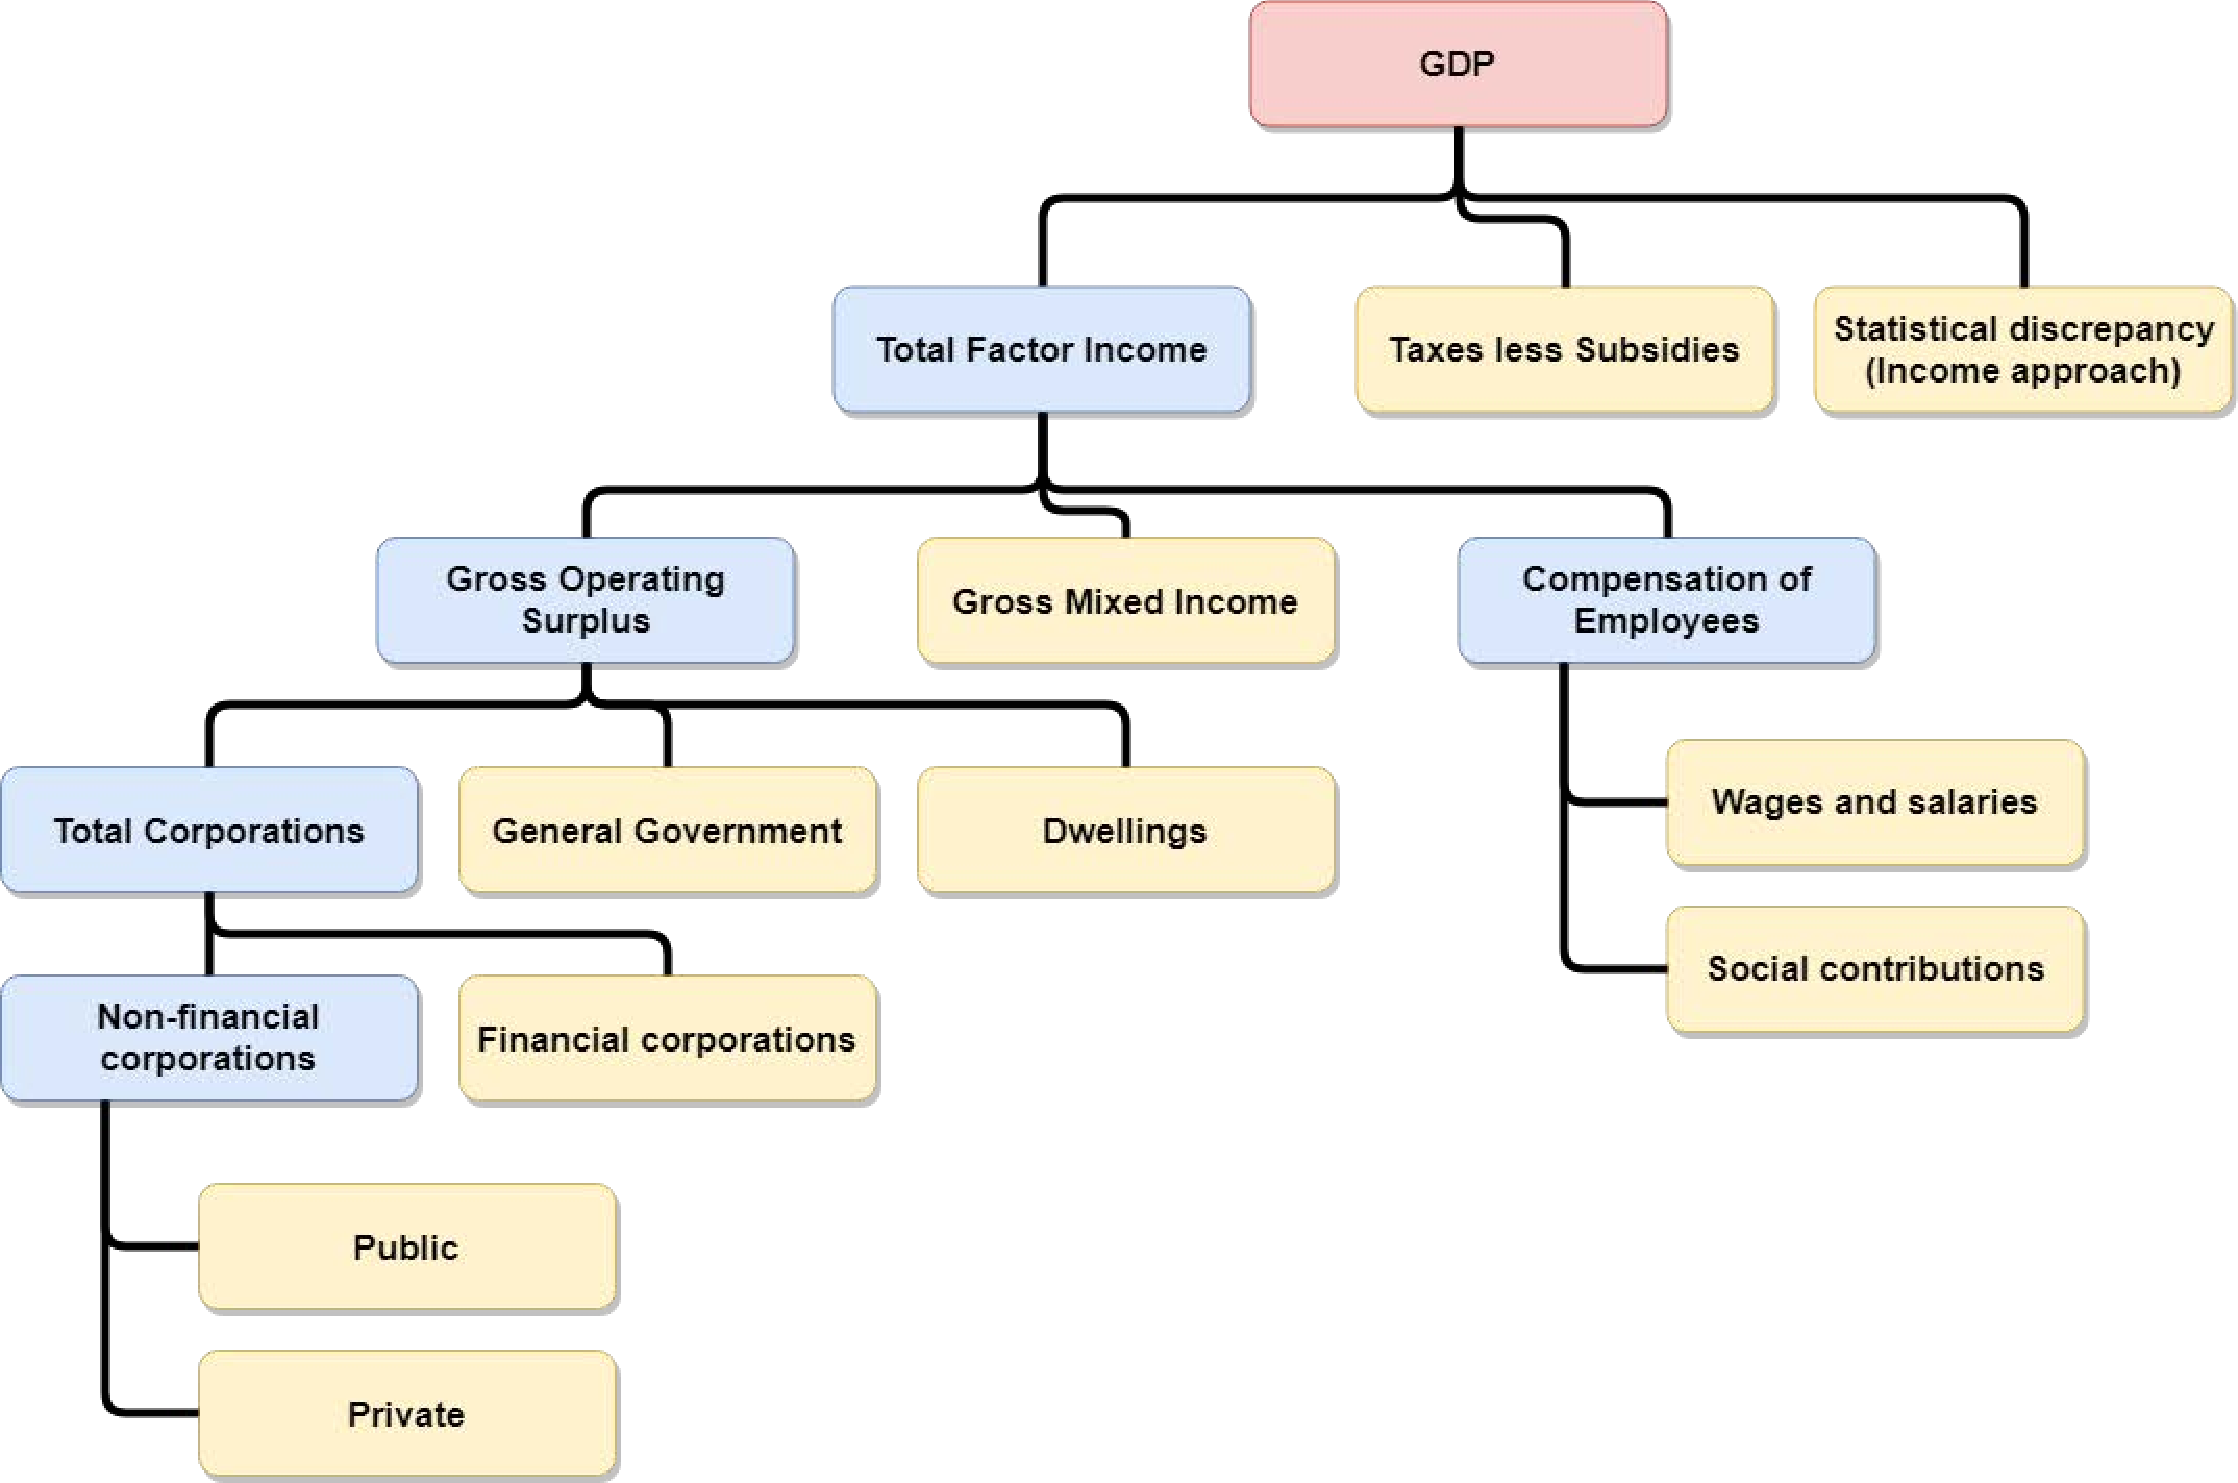
\includegraphics[width=.9\textwidth]{Figs/Hierarchical-structures/IncomeApproach.pdf}
	\caption{Hierarchical structure of the income approach for GDP\@. The pink cell contains GDP the most aggregate series. The blue cells contain intermediate-level series and the yellow cells correspond to the most disaggregate bottom-level series.}\label{fig:GDP_I}
\end{figure}

\subsubsection*{Expenditure approach}

\begin{figure}
	\centering	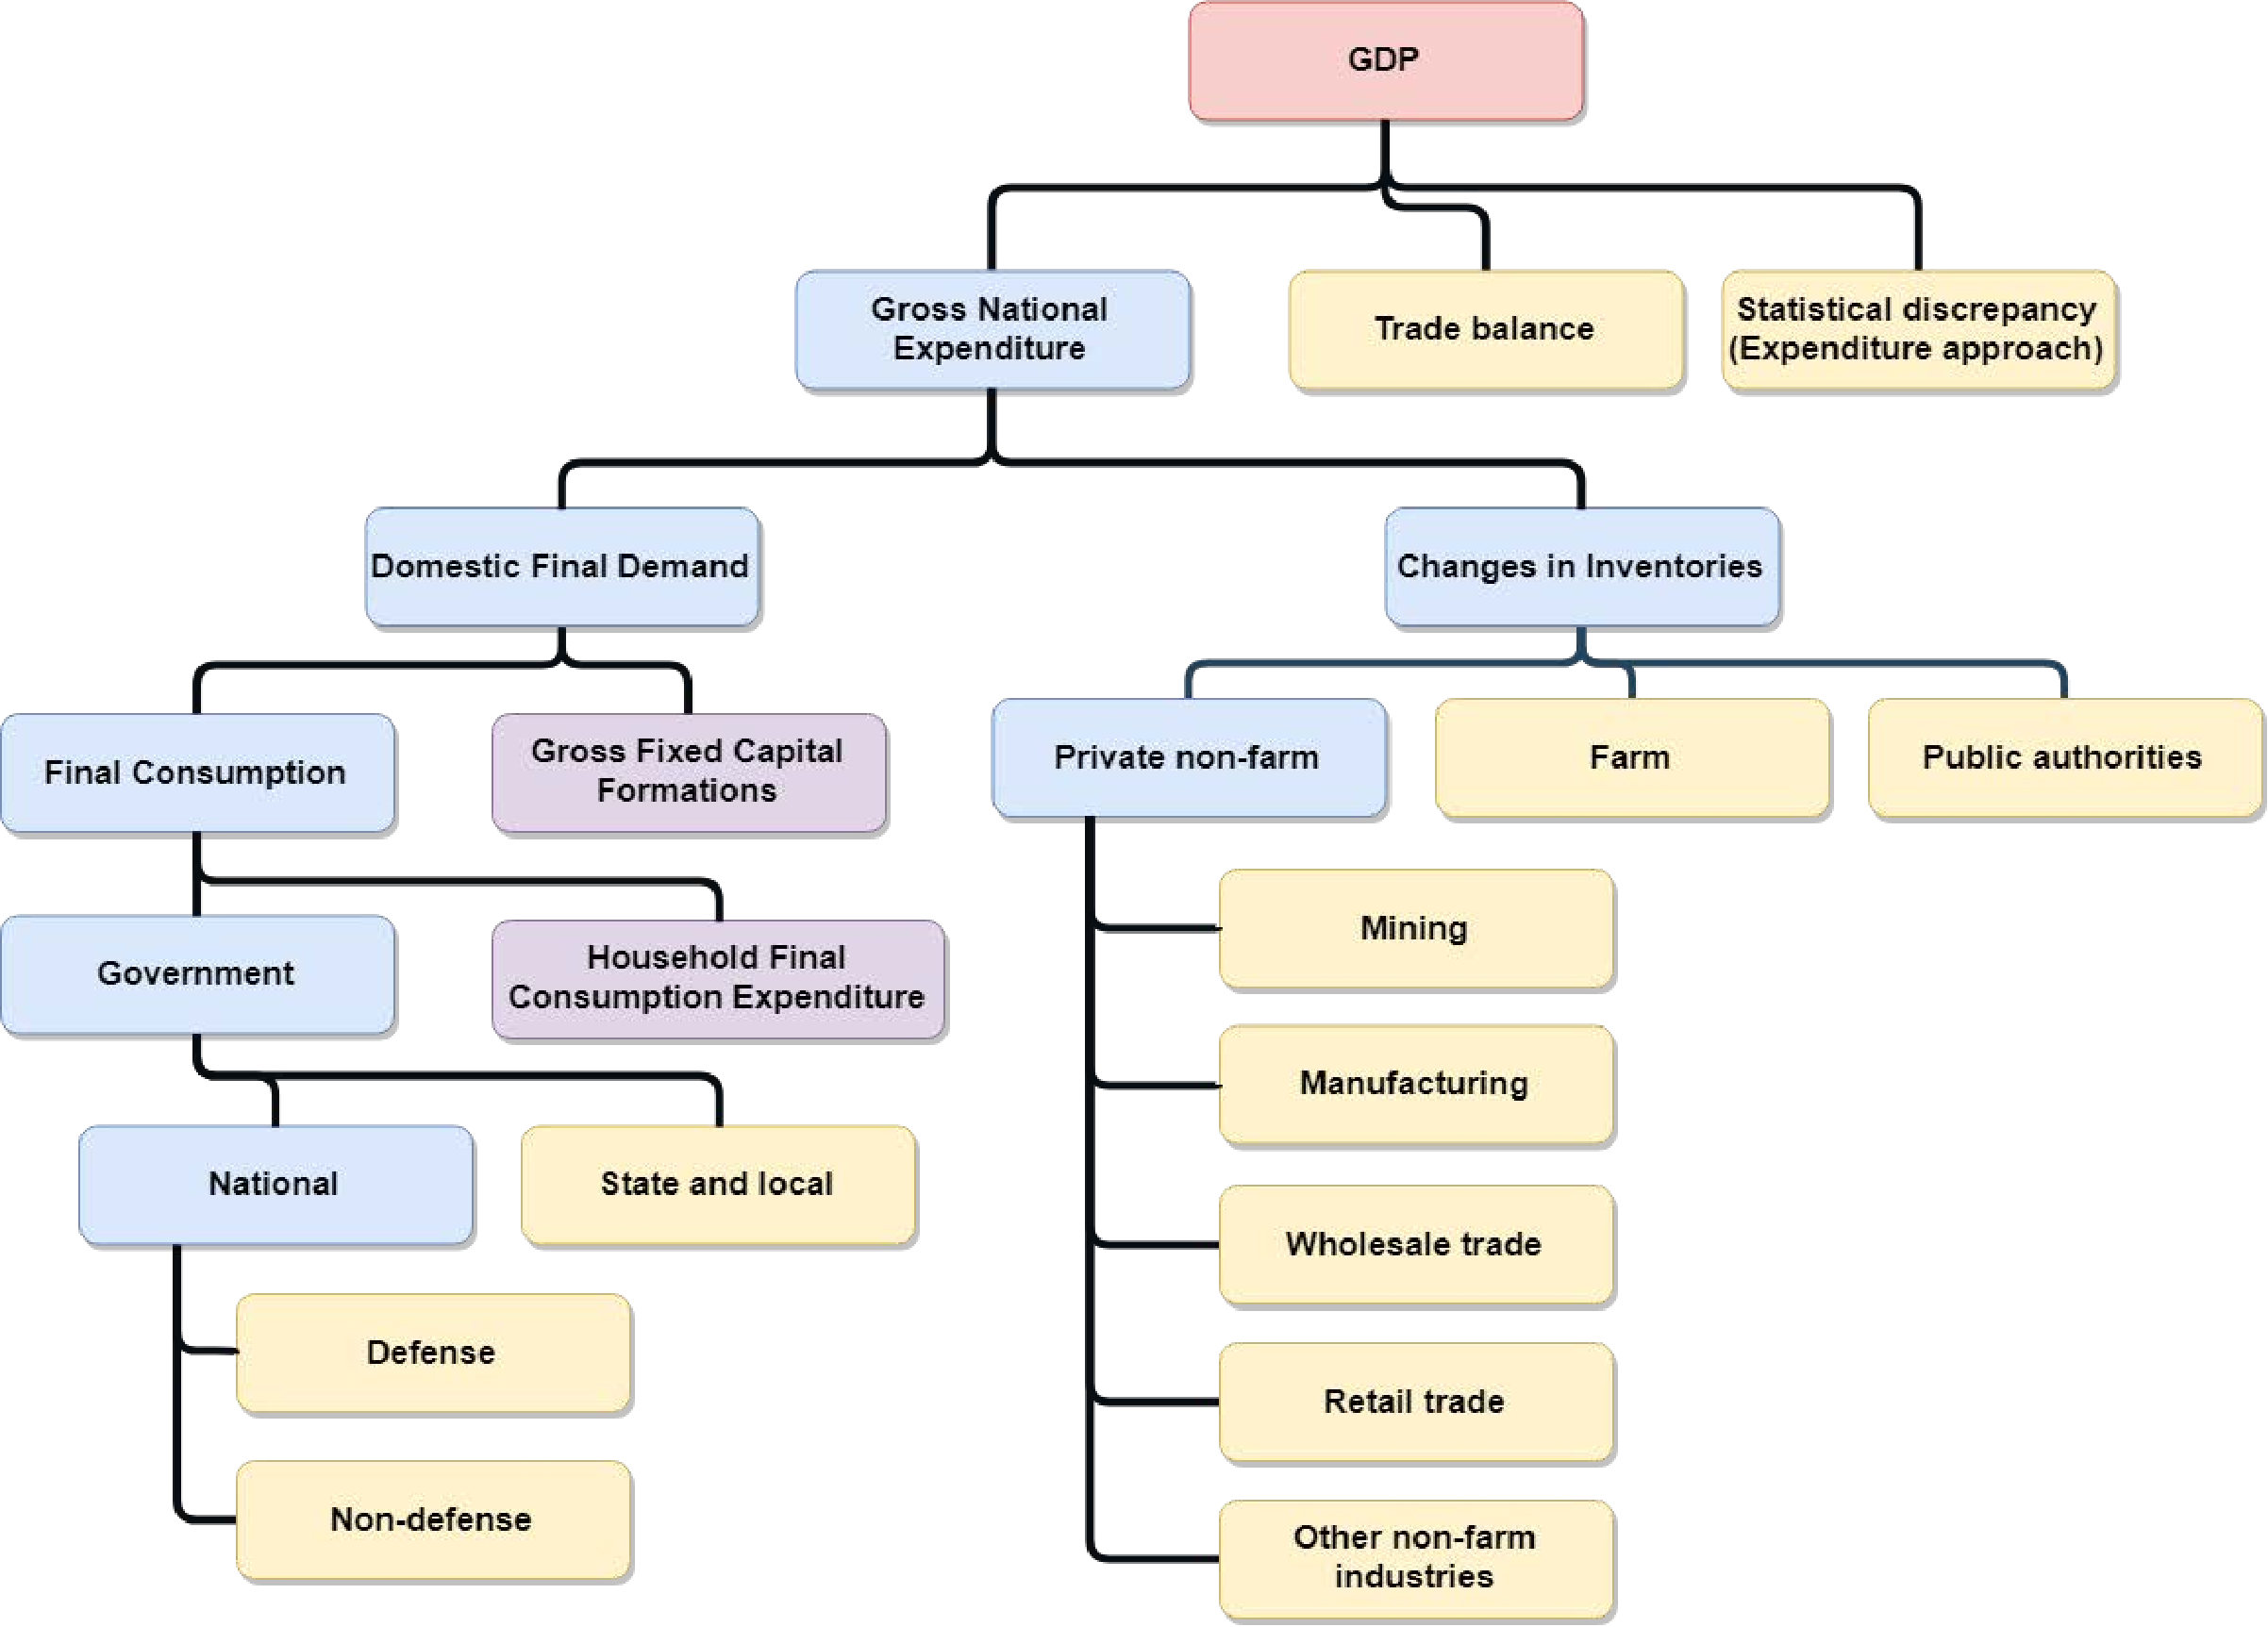
\includegraphics[width=.9\textwidth]{Figs/Hierarchical-structures/ExpenditureApproach.pdf}
	\caption{Hierarchical structure of the expenditure approach for GDP\@. The pink cell contains GDP, the most aggregate series. The blue and purple cells contain intermediate-level series with the series in the purple cells further disaggregated in Figures~\ref{fig:GFCF} and~\ref{fig:HFCE}. The yellow cells contain the most disaggregate bottom-level series.}\label{fig:GDP_E}
	\centering
	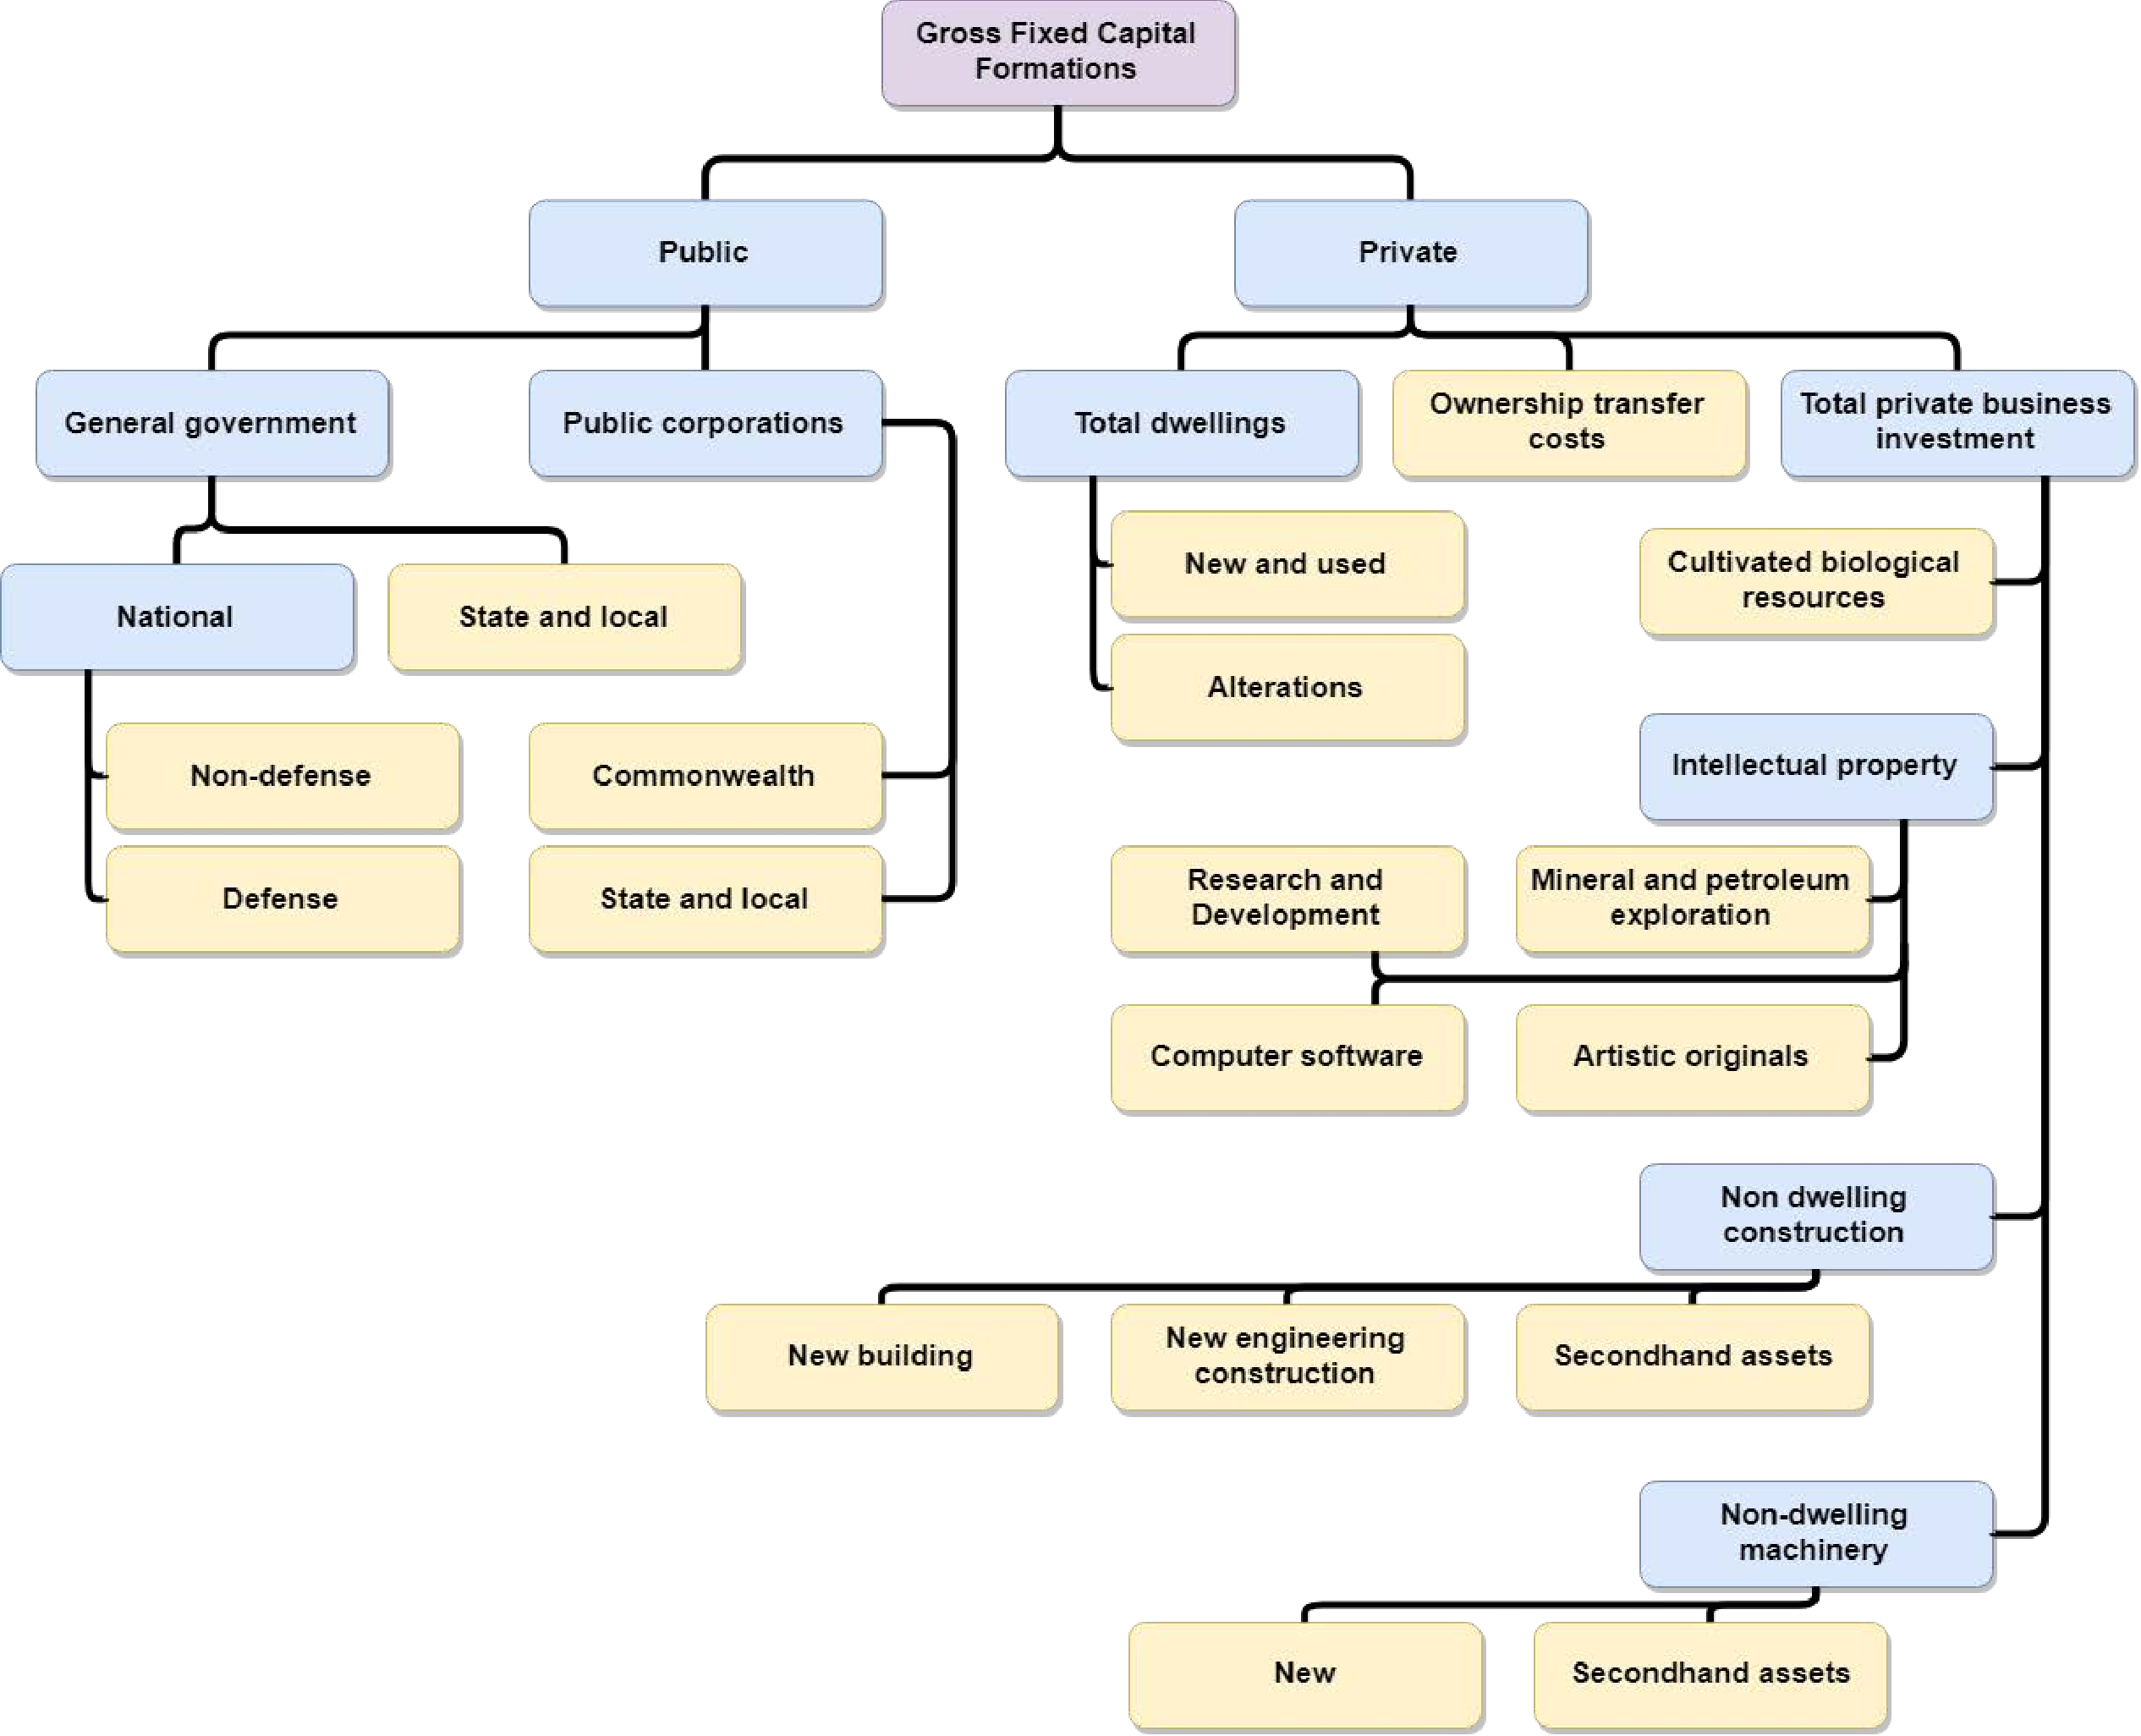
\includegraphics[width=.9\textwidth]{Figs/Hierarchical-structures/GFCF.pdf}
	\caption{Hierarchical structure for Gross Fixed Capital Formations under the expenditure approach for GDP, continued from \autoref{fig:GDP_E}. Blue cells contain intermediate-level series and the yellow cells correspond to the most disaggregate bottom-level series.}\label{fig:GFCF}
\end{figure}

In the expenditure approach, GDP is calculated as the aggregation of final consumption expenditure, gross fixed capital formation (GFCF), changes in inventories of finished goods, work-in-progress and raw materials and the value of exports less imports of the goods and services \citep{ABS2015}. The underline equation is:
\begin{align*}
	\textit{GDP}
	 & = \textit{Final consumption expenditure}
     + \textit{Gross fixed capital formation} \\
	 & + \textit{Changes in inventories}
     + \textit{Trade balance}
     + \textit{Statistical discrepancy (E)}.
\end{align*}
Figures~\ref{fig:GDP_E}, \ref{fig:GFCF} and~\ref{fig:HFCE} show the full hierarchical structure capturing all components aggregated to form GDP using the expenditure approach. The hierarchy has three levels of aggregation below the top-level, with a total of $n=80$ series across the whole structure and $m=53$ series at the bottom level. Descriptions of each series in these hierarchies along with the series ID assigned by the ABS are given in the Tables~\ref{Tab: Income-hierarchy}, \ref{Tab:Expenditure-hierarchy-1}, \ref{Tab:Expenditure-hierarchy-2} and~\ref{Tab:Expenditure-hierarchy-3} in the Appendix.

\begin{figure}[!t]
	\centering
	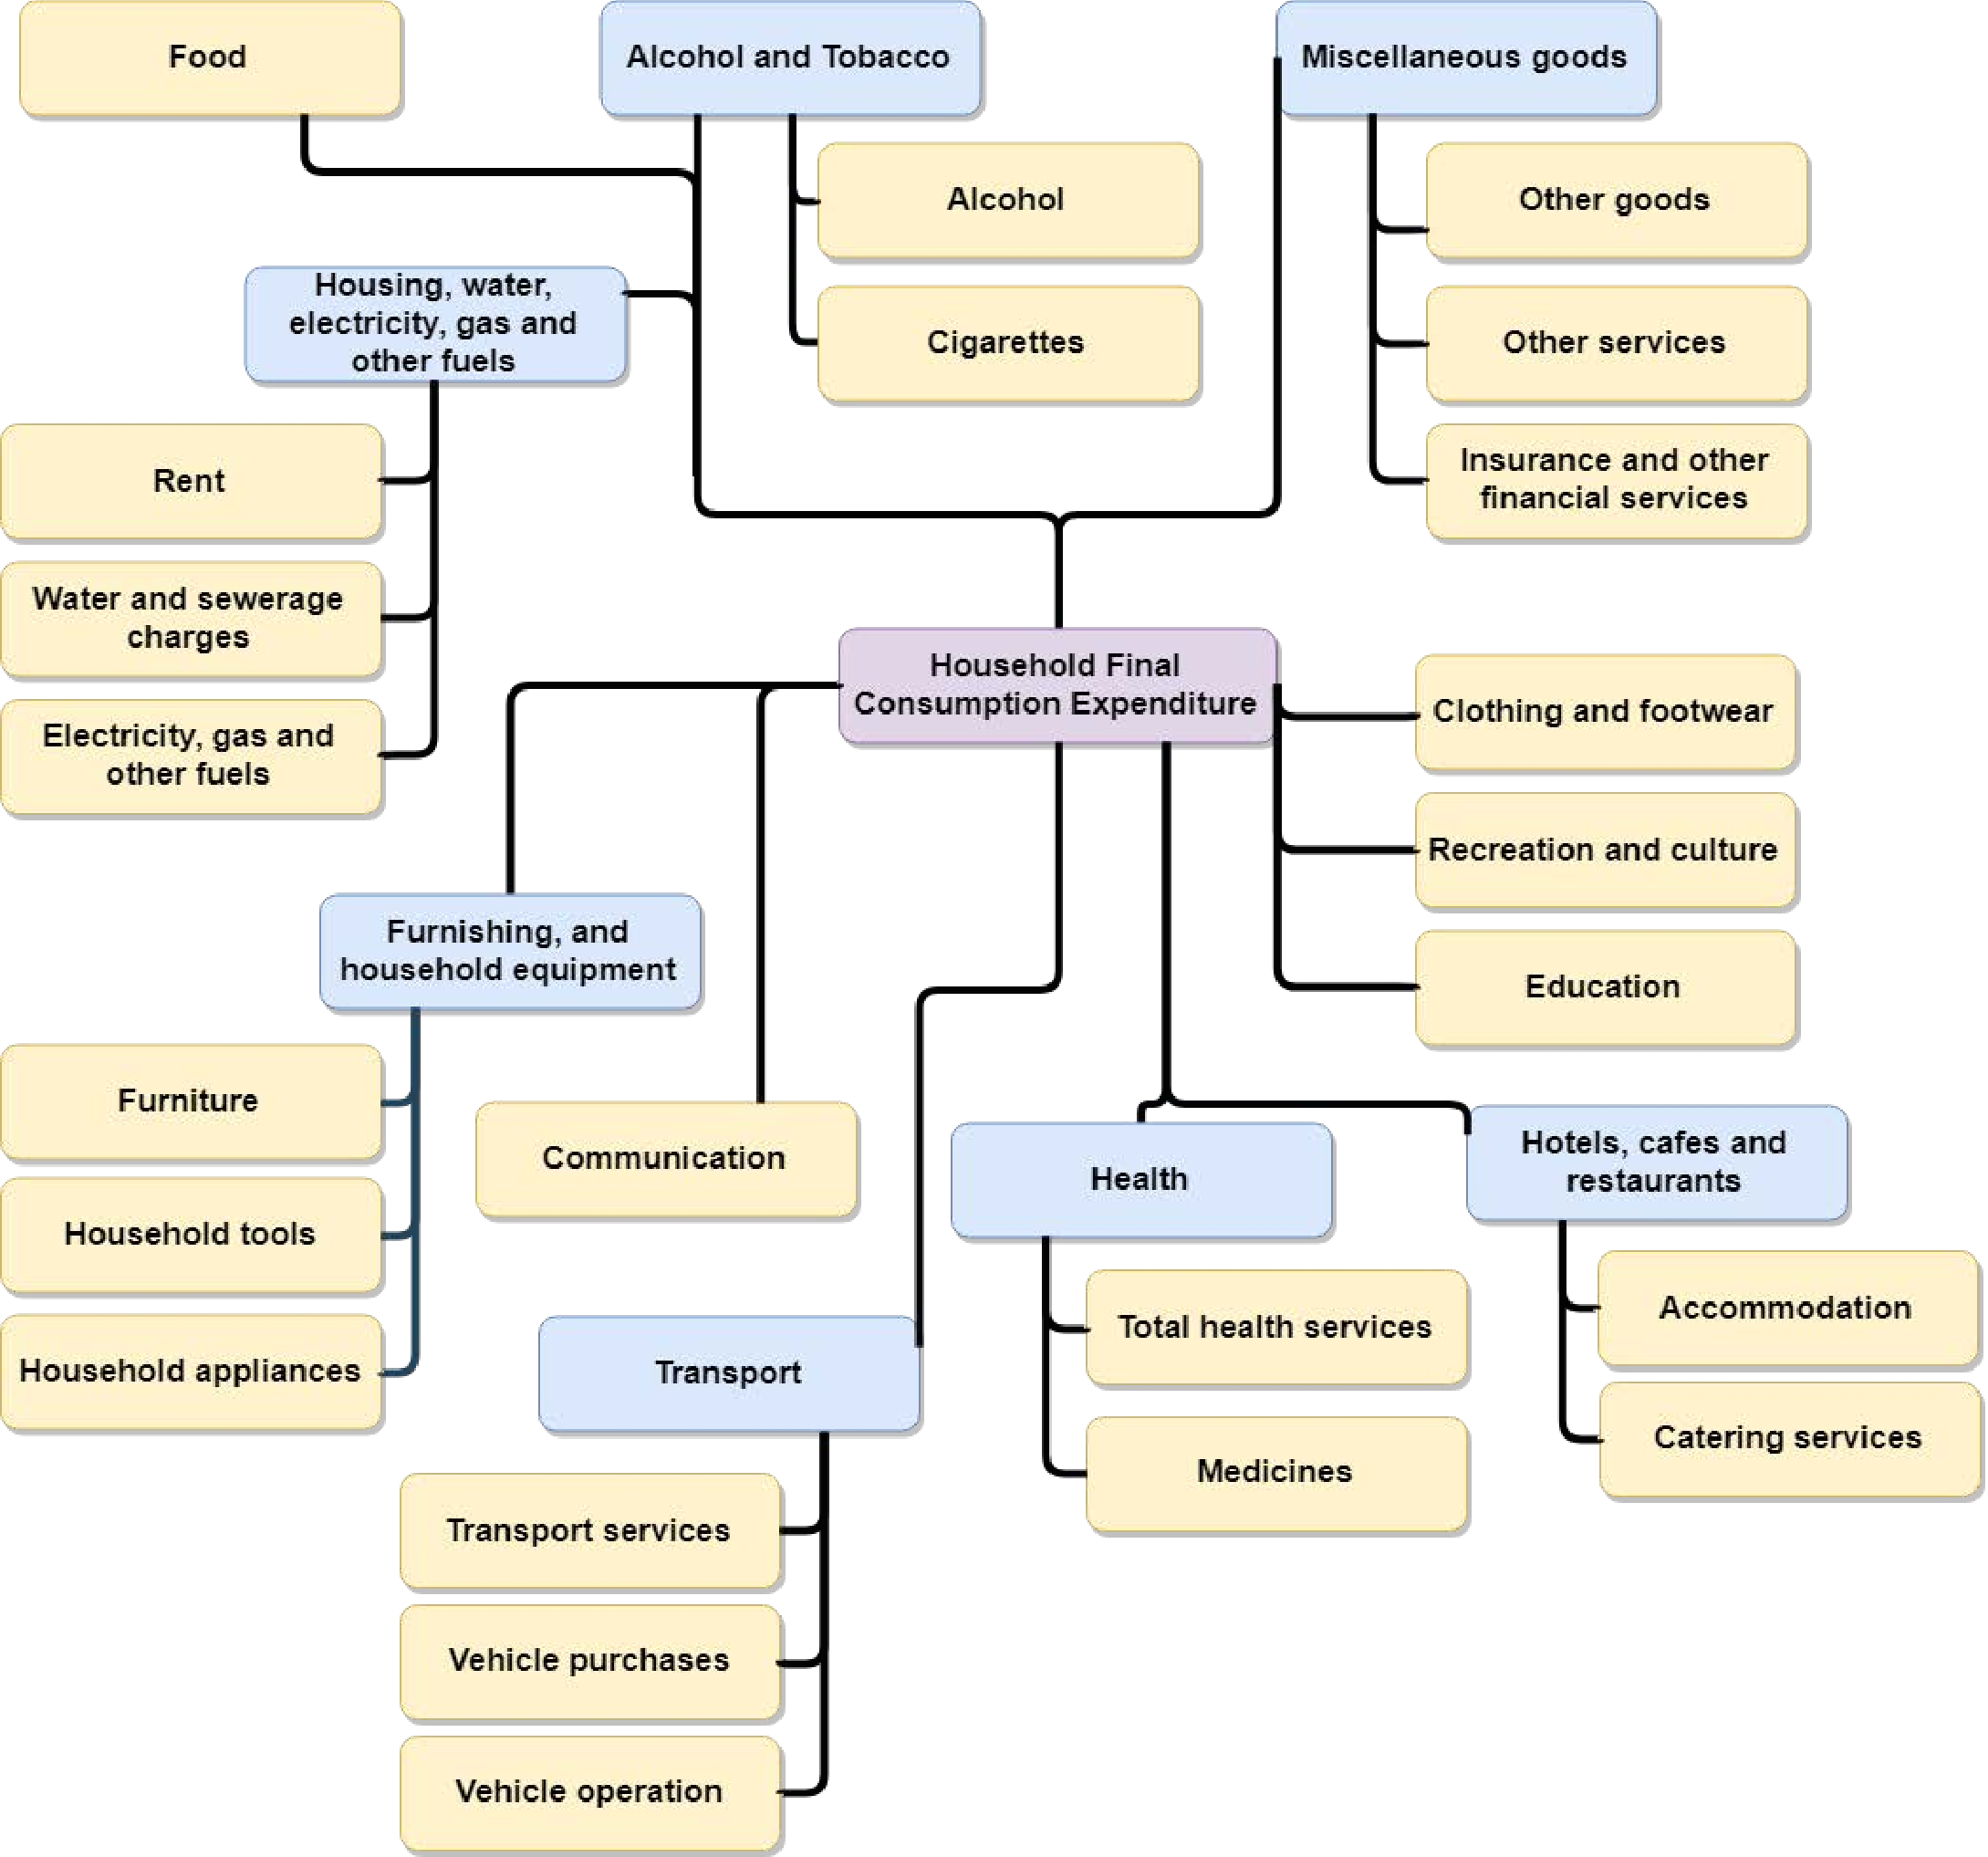
\includegraphics[width=.9\textwidth]{Figs/Hierarchical-structures/HFCE.pdf}
	\caption{Hierarchical structure for Household Final Consumption Expenditure under the expenditure approach for GDP, continued from \autoref{fig:GDP_E}. Blue cells contain intermediate-level series and the yellow cells correspond to the most disaggregate bottom-level series.}\label{fig:HFCE}
\end{figure}

\autoref{fig:TSplots-INC-EXP} displays time series from the income and expenditure approaches. The top panel shows the most aggregate GDP series. The panels below show series from lower levels for the income hierarchy (left panel) and the expenditure hierarchy (right panel). The plots show the diverse features of the time series with some displaying positive and others negative trending behaviour, some showing no trends but possibly a cycle, and some having a strong seasonal component. These highlight the need to account for and model all information and diverse signals from each series in the hierarchy, which can only be achieved through a forecast reconciliation approach.

\begin{figure}
	\centering
	\small
	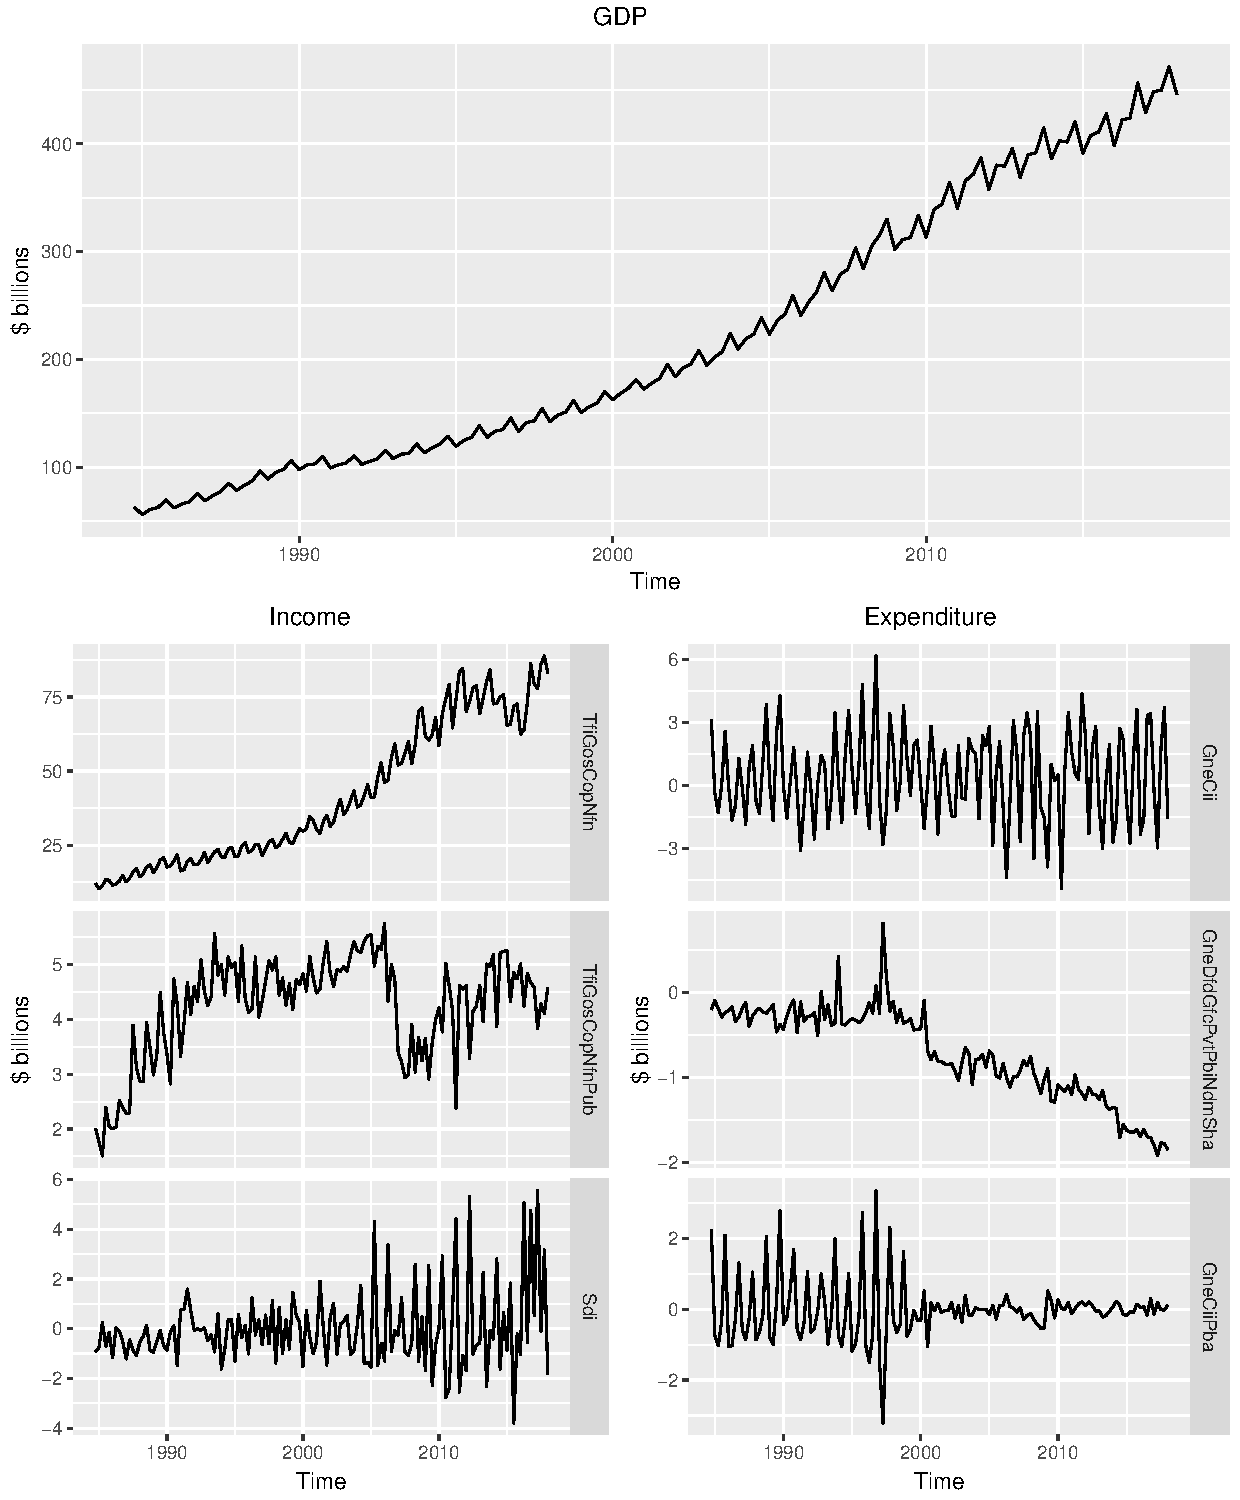
\includegraphics[width = \textwidth]{Figs/TS-plots/TSplots-INC-EXP.pdf}
	\caption{Time plots for series from different levels of income and expenditure hierarchies.}\label{fig:TSplots-INC-EXP}
\end{figure}

\section{Empirical application methodology}\label{sec:meth}

We now demonstrate the potential for reconciliation methods to improve forecast accuracy for Australian GDP\@. We consider forecasts from $h=1$ quarter ahead up to $h=4$ quarters ahead using an \emph{expanding} window. First, the training sample is set from 1984:Q4 to 1994:Q3 and forecasts are produced for 1994:Q4 to 1995:Q3. Then the training window is expanded by one quarter at a time, i.e.\ from 1984:Q4 to 2017:Q4 with the final forecasts produced for the last available observation in 2018:Q1. This leads to 94 1-step-ahead, 93 2-steps-ahead, 92 3-steps-ahead and 91 4-steps-ahead forecasts available for evaluation.

\subsection{Models}

The first task in forecast reconciliation is to obtain base forecasts for all series in the hierarchy. In the case of the income approach, this necessitates forecasting $n=16$ separate time series while in the case of the expenditure approach, forecasts for $n=80$ separate time series must be obtained. Given the diversity in these time series discussed in \autoref{sec:data}, we focus on an approach that is fast but also flexible. We consider simple univariate ARIMA models, where model order is selected via a combination of unit root testing and the AIC using an algorithm developed by \citet{HK08} and implemented in the \verb|auto.arima()| function in \citet{Rforecast}. A similar approach was also undertaken using the ETS framework to produce base forecasts \citep{expsmooth08}. This had minimal impact on our conclusions with respect to forecast reconciliation methods, and in most cases ARIMA forecasts were found to be more accurate than ETS forecasts. Consequently for brevity, we have excluded presenting the results for ETS models. However, these are available from github \footnote {The relevant github repository is \href{https://github.com/PuwasalaG/Hierarchical-Book-Chapter}{PuwasalaG/Hierarchical-Book-Chapter}} and are discussed in detail in \cite{gamakumara2019phd}. We note that a number of more complicated approaches could have been used to obtain base forecasts including multivariate models such as vector autoregressions, and models and methods that handle a large number of predictors such as factor models or least angle regression. However, \citet{PanEtAl2019} show that univariate ARIMA models are highly competitive for forecasting Australian GDP even compared to these methods, and in any case our primary motivation is to demonstrate the potential of forecast reconciliation.

The hierarchical forecasting approaches we consider are bottom-up, OLS, WLS with variance scaling and the MinT(Shrink) approach. The MinT(Sample) approach was also used but due to the size of the hierarchy, forecasts reconciled via this approach were less stable. Finally, all forecasts (both base and coherent) are compared to a seasonal \naive benchmark \citep{HynAth2018}; i.e.\ the forecast for GDP (or one of its components) is the realised GDP in the same quarter of the previous year. The \naive forecasts are by construction coherent and therefore do not need to be reconciled.

\subsection{Evaluation}

For evaluating point forecasts we consider two metrics, the Mean Squared Error (MSE) and the Mean Absolute Scaled Error (MASE) calculated over the expanding window. The absolute scaled error is defined as
\begin{equation*}
	q_{T+h} = \frac{|\breve{e}_{T+h|T}|}{(T-4)^{-1}\sum_{t=5}^{T}|y_t - y_{t-4}|}\,,
\end{equation*}
where $\breve{e}_{t+h}$ is the difference between any forecast and the realisation\footnote{Breve is used instead of a hat or tilde to denote that this can be the error for either a base or reconciled forecast.}, and $4$ is used due to the quarterly nature of the data. An advantage of using MASE is that it is a scale independent measure. This is particularly relevant for hierarchical time series, since aggregate series by their very nature are on a larger scale than disaggregate series. Consequently, scale dependent metrics may unfairly favour methods that perform well for the aggregate series but poorly for disaggregate series. For more details on different point forecast accuracy measures, refer to Chapter 3 of \citet{HynAth2018}.

Forecast accuracy of probabilistic forecasts can be evaluated using scoring rules \citep{Gneiting2014}. Let $\breve{F}$ be a probabilistic forecast and let $\breve{\bm{y}}\sim \breve{F}$ where a breve is again used to denote that either base forecasts or coherent forecasts can be evaluated. The accuracy of multivariate probabilistic forecasts will be measured by the energy score given by
\begin{equation*}
	eS(\breve{F}_{T+h|T},\bm{y}_{T+h}) =
	\E_{\breve{F}}\|\breve{\bm{y}}_{T+h}-\bm{y}_{T+h}\|^\alpha
	-\frac{1}{2}\E_{\breve{F}}\|\breve{\bm{y}}_{T+h}-\breve{\bm{y}}^*_{T+h}\|^\alpha\,,
\end{equation*} where $\bm{y}_{T+h}$ is the realisation at time $T+h$, and $\alpha\in (0,2]$. We set $\alpha=1$, noting that other values of $\alpha$ give similar results. The expectations can be evaluated numerically as long as a sample from $\breve{F}$ is available, which is the case for all methods we employ. An advantage of using energy scores is that in the univariate case it simplifies to the commonly used cumulative rank probability score (CRPS) given by
\begin{equation*}
	\text{CRPS}(\breve{F}_i,y_{i,T+h}) = \E_{\breve{F}_i}|\breve{y}_{i,T+h}-y_{i,T+h}| - \frac{1}{2}\E_{\breve{F}_i}|\breve{y}_{i,T+h}-\breve{y}^*_{i,T+h}|,
\end{equation*}
where the subscript $i$ is used to denote that CRPS measures forecast accuracy for a single variable in the hierarchy.

Alternatives to the energy score were also considered, namely log scores and variogram scores. The log score was disregarded since \citet{GamEtAl2018} prove that the log score is improper with respect to the class of incoherent probabilistic forecasts when the true DGP is coherent. The variogram score gave similar results to the energy score;  these results are omitted for brevity but are available from these are available from github and are discussed in detail in \cite{gamakumara2019phd}


\section{Results}\label{sec:results}

\subsection{Base forecasts}

Due to the different features in each time series, a variety of ARIMA and seasonal ARIMA models were selected for generating base forecasts. For example, in the income hierarchy, some series require seasonal differencing while other did not. Furthermore the AR orders vary from 0--3, the MA orders from 0--2, and their seasonal counterparts SAR from 0--2 and SMA from 0--1. \autoref{fig: NaiveVsBase_MSE} compares the accuracy of the ARIMA base forecasts to the seasonal \naive forecasts over different forecast horizons. The panels on the left show results for the Income hierarchy while the panels on the right show the results for the Expenditure hierarchy. The top panels summarise results over all series in the hierarchy, i.e.\ we calculate the MSE for each series and then average over all series. The bottom panels show the results for the aggregate level GDP.

The clear result is that base forecasts are more accurate than the \naive forecasts, however as the forecasting horizon increases, the differences become smaller. This is to be expected since the \naive model here is a seasonal random walk, and for horizons $h<4$, forecasts from an ARIMA model are based on more recent information. Similar results are obtained when MASE is used as the metric for evaluating forecast accuracy.

One disadvantage of the base forecasts relative to the \naive forecasts is that base forecasts are not coherent. As such we now turn our attention to investigating whether reconciliation approaches can lead to further improvements in forecast accuracy relative to the base forecasts.

\begin{figure}
	\centering
	\small
	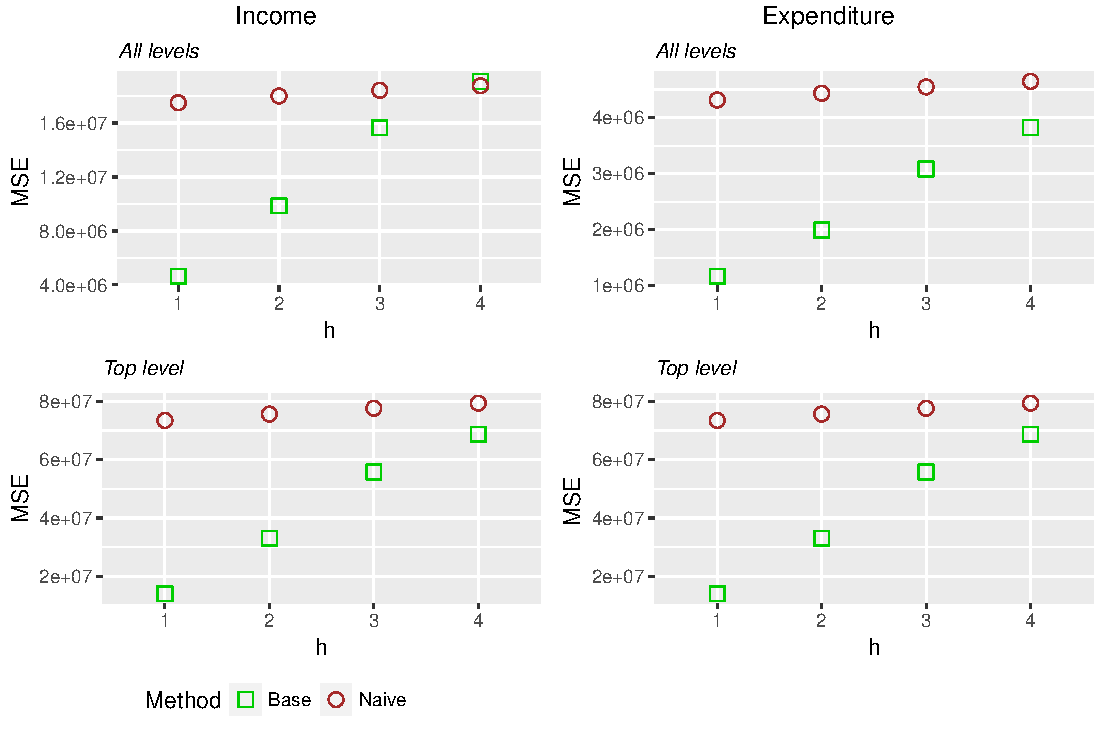
\includegraphics[width=\textwidth]{Figs/Results/NaiveVsBase_MSE.pdf}
	\caption{Mean squared errors for \naive and ARIMA base forecasts. Top panels refer to results summarised over all series while bottom panels refer to results for the top-level GDP series. Left panels refer to the income hierarchy and right panels to the expenditure hierarchy.}\label{fig: NaiveVsBase_MSE}
\end{figure}

\subsection{Point Forecast Reconciliation}

We now turn our attention to evaluating the accuracy of point forecasts obtained using the different reconciliation approaches as well as the single-level bottom-up approach. All results in subsequent figures are presented as the percentage changes in a forecasting metric relative to base forecasts, a measure known in the forecasting literature as \emph{skill scores}. Skill scores are computed such that positive values represent an improvement in forecasting accuracy over the base forecasts while negative values represent a deterioration.

\begin{figure}
	\centering
	\small
	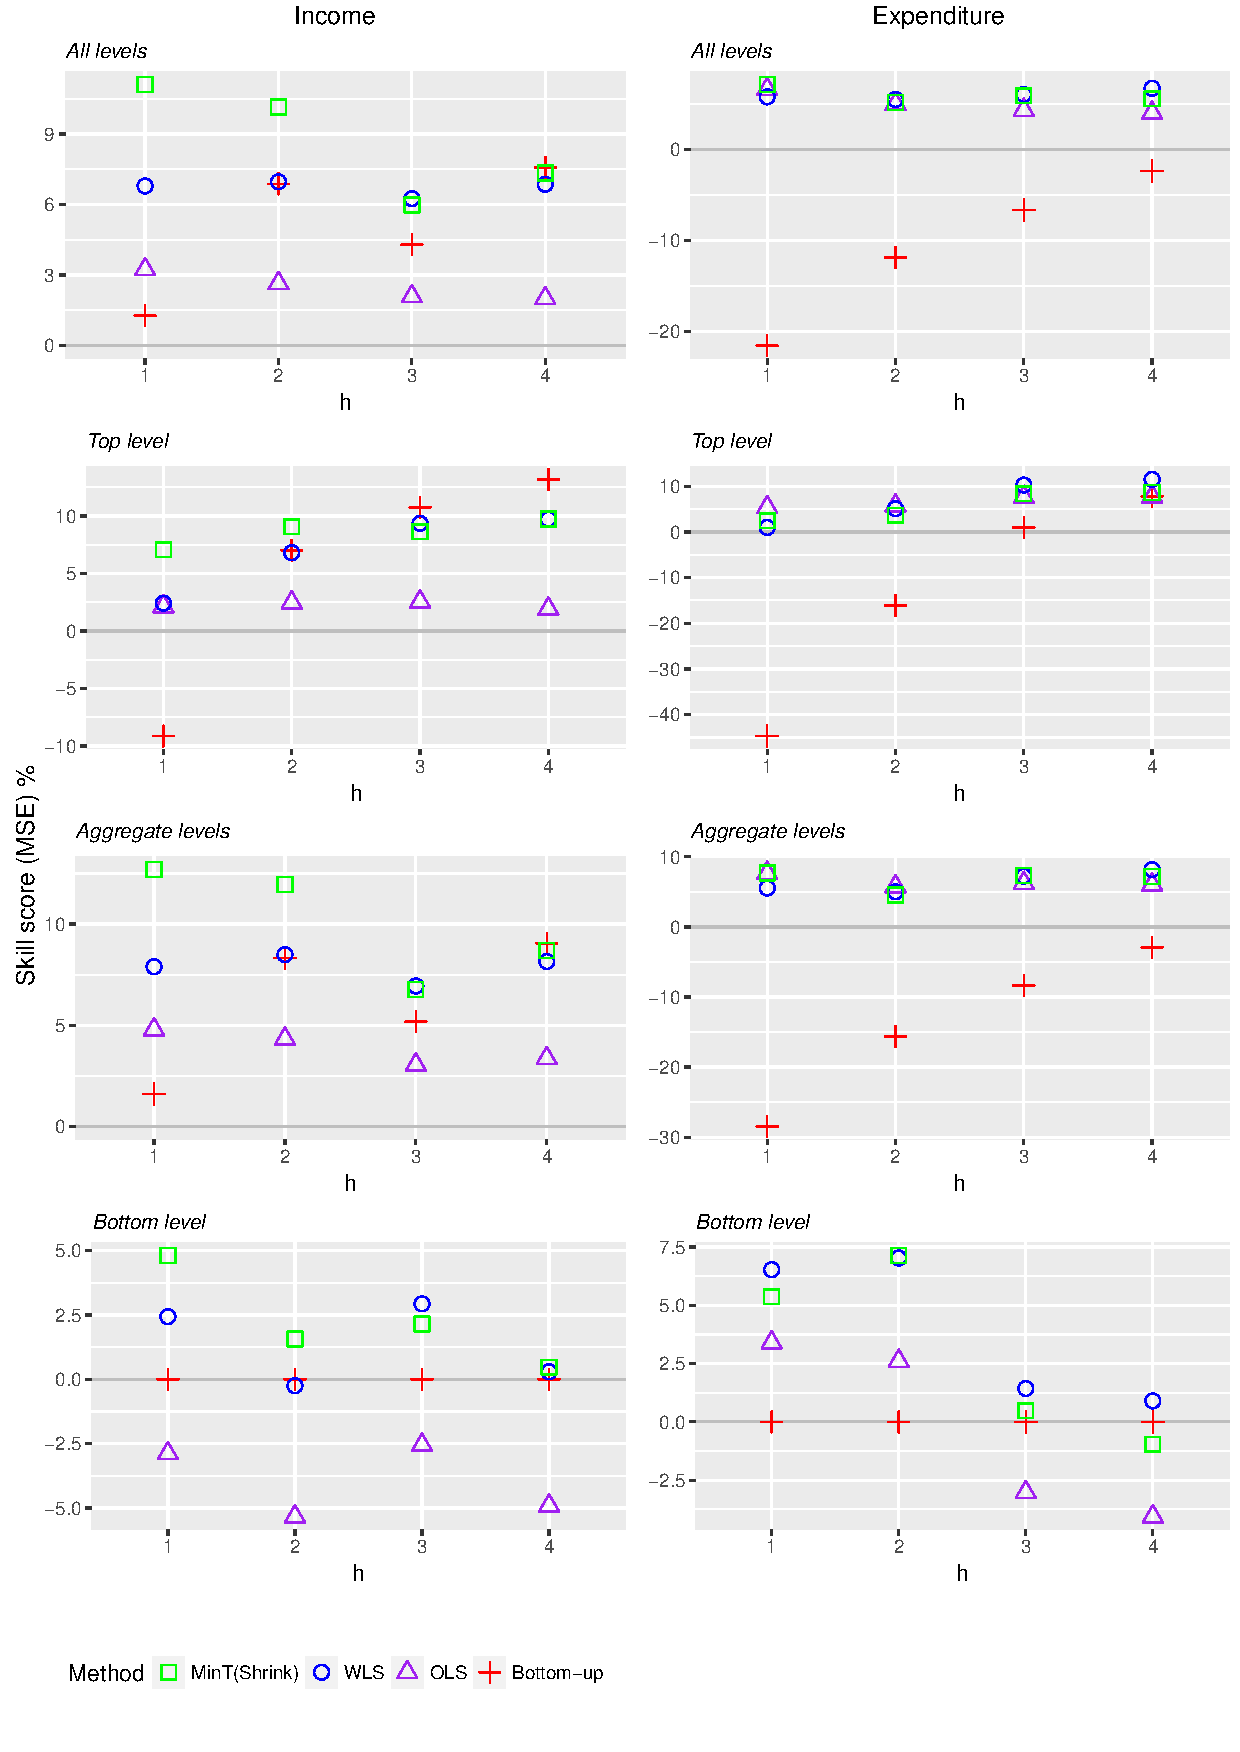
\includegraphics[width=\textwidth]{Figs/Results/PointF_MSE.pdf}
	\caption{Skill scores for point forecasts from alternative methods (with reference to base forecasts) using MSE\@. The left panels refer to the income hierarchy while the right panels refer to the expenditure hierarchy. The first row refers to results summarised over all series, the second row to top-level GDP series, the third row to aggregate levels, and the last row to the bottom level.}
	\label{fig: PointF_MSE}
\end{figure}

\begin{figure}
	\centering
	\small
	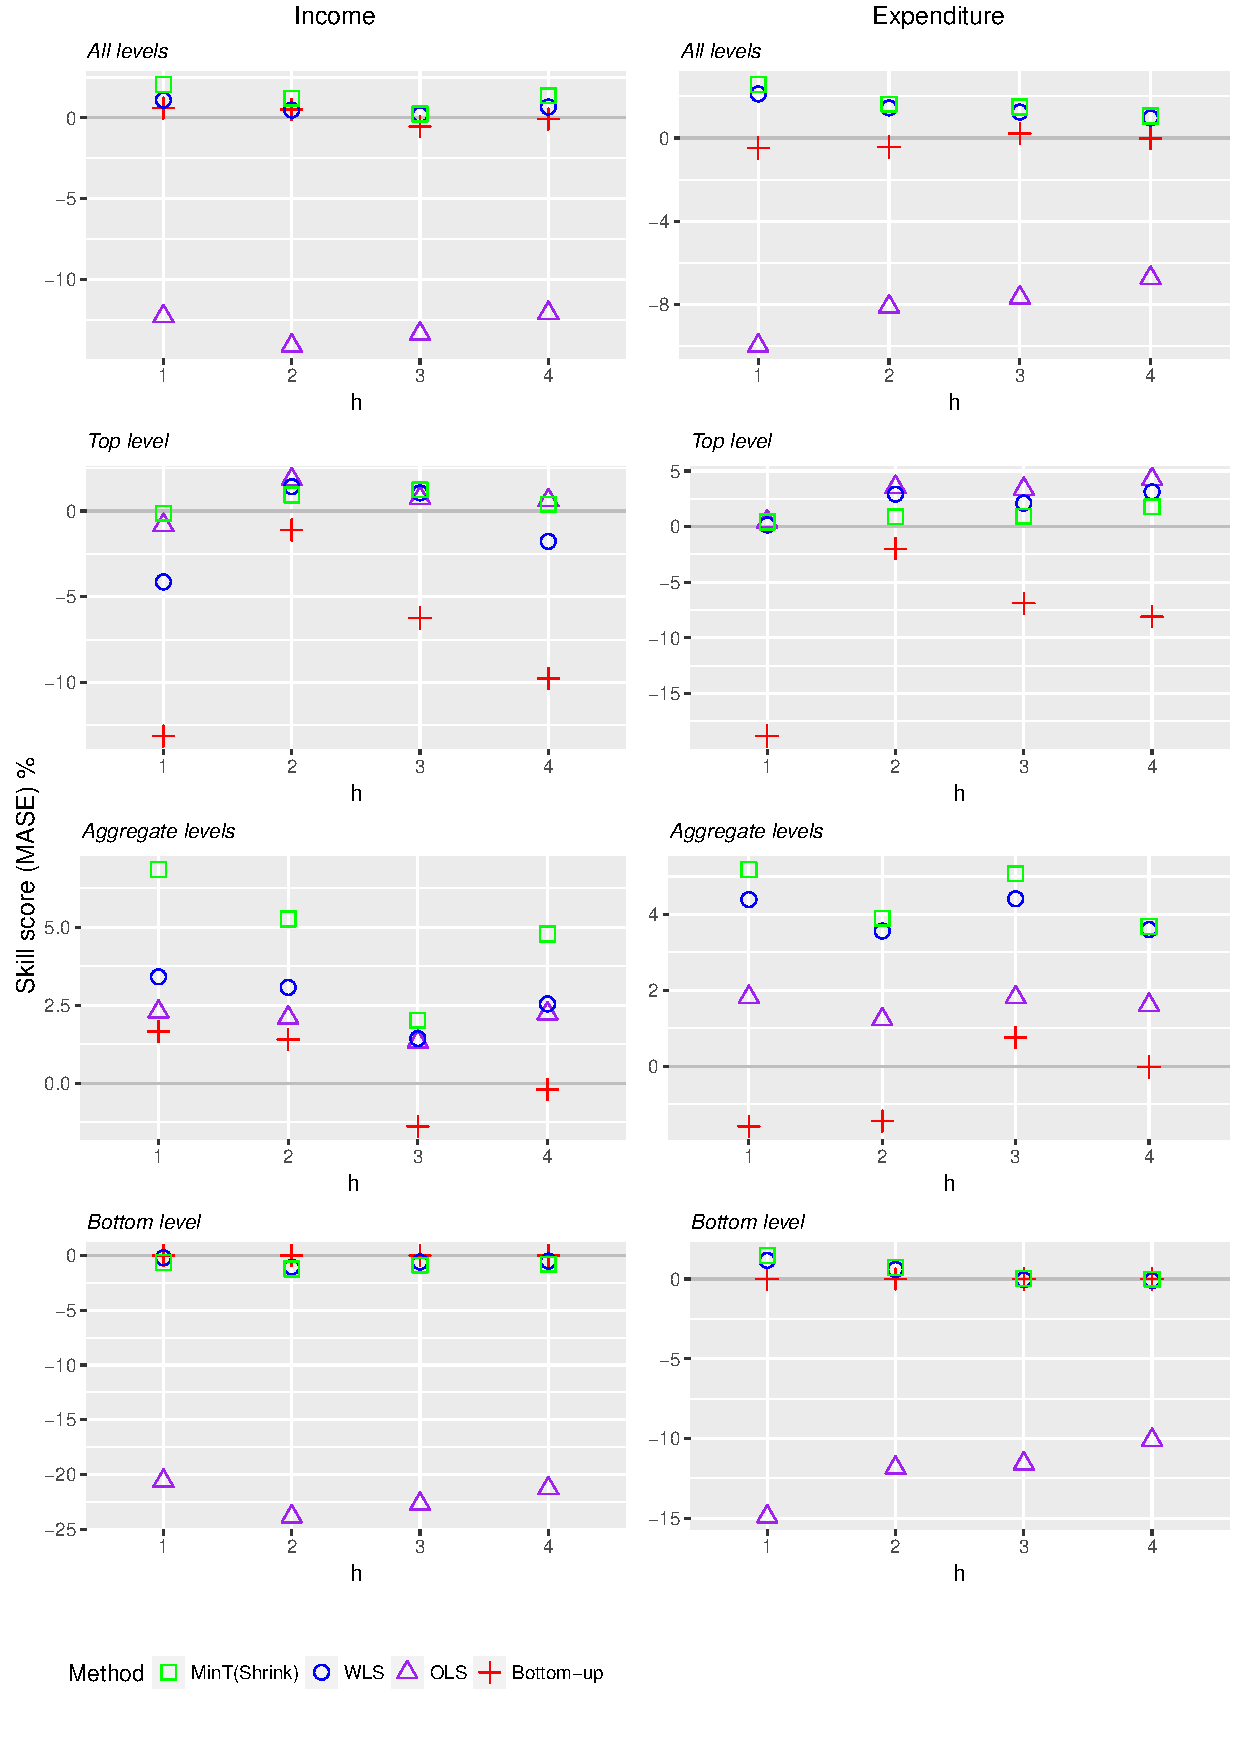
\includegraphics[width=\textwidth]{Figs/Results/PointF_MASE.pdf}
	\caption{Skill scores for point forecasts from different reconciliation methods (with reference to base forecasts) using MASE\@. The left two panels refer to the income hierarchy and the right two panels to the expenditure hierarchy. The first row refers to results summarised over all series, the second row to top-level GDP series, the third row to aggregate levels, and the last row to the bottom level.}
	\label{fig: PointF_MASE}
\end{figure}

Figures~\ref{fig: PointF_MSE} and~\ref{fig: PointF_MASE} show skill scores using MSE and MASE respectively. The top row of each figure shows skill scores based on averages over all series. We conclude that reconciliation methods generally improve forecast accuracy relative to base forecasts regardless of the hierarchy used, the forecasting horizon, the forecast error measure or the reconciliation method employed. We do however note that while all reconciliation methods improve forecast performance, MinT(Shrink) is the best forecasting method in most cases.

To further investigate the results we break down the skill scores by different levels of each hierarchy. The second row of Figures~\ref{fig: PointF_MSE} and~\ref{fig: PointF_MASE} shows the skill scores for a single series, namely GDP which represents the top-level of both hierarchies. The third row shows results for all series excluding those of the bottom level, while the final row shows results for the bottom-level series only. Here, we see two general features. The first is that OLS reconciliation performs poorly on the bottom-level series, and the second is that bottom-up performs relatively poorly on aggregate series. The two features are particularly exacerbated for the larger expenditure hierarchy. These results are consistent with other findings in the forecast reconciliation literature \citep[see for instance][]{AthEtAl2017,WicEtAl2019}

\subsection{Probabilistic Forecast Reconciliation}

\begin{figure}[!b]
	\centering
	\small
	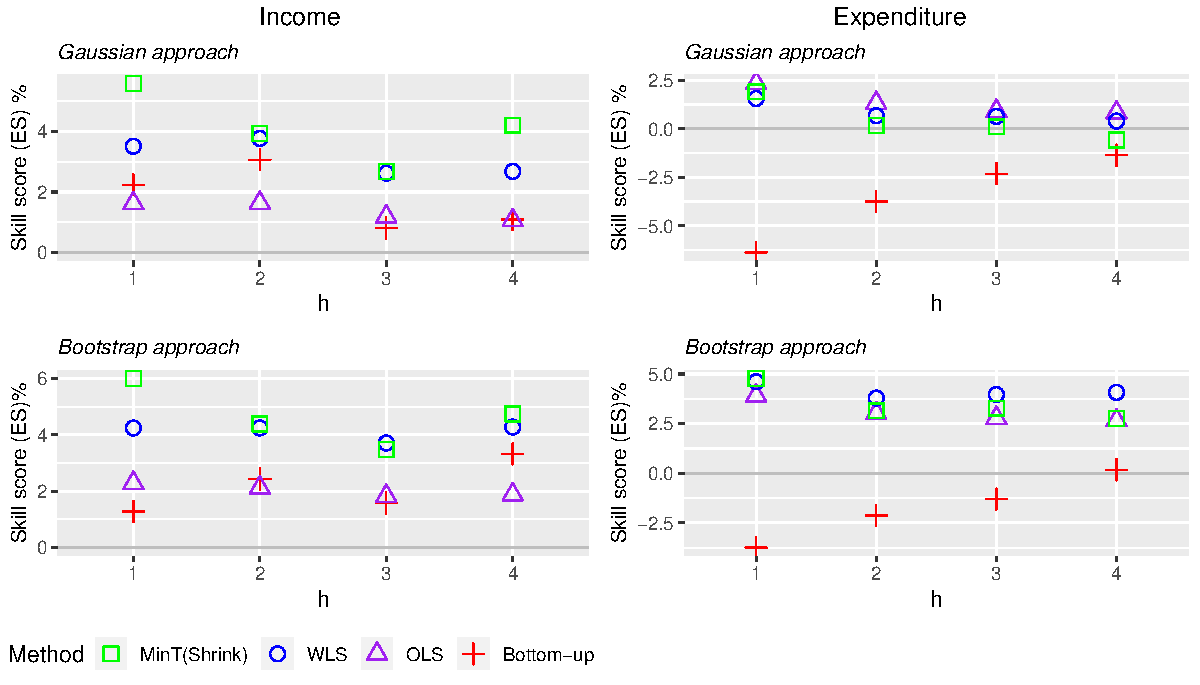
\includegraphics[width=\textwidth]{Figs/Results/ProbF_MultivS.pdf}
	\caption{Skill scores for multivariate probabilistic forecasts from different reconciliation methods (with reference to base forecasts) using energy scores. The top panels refer to the results for the Gaussian approach and the bottom panels to the non-parametric bootstrap approach. Left panels refer to the income hierarchy and right panels to the expenditure hierarchy.}
	\label{fig: Prob-forecasts-SS_ES}
\end{figure}

\begin{figure}
	\centering
	\small
	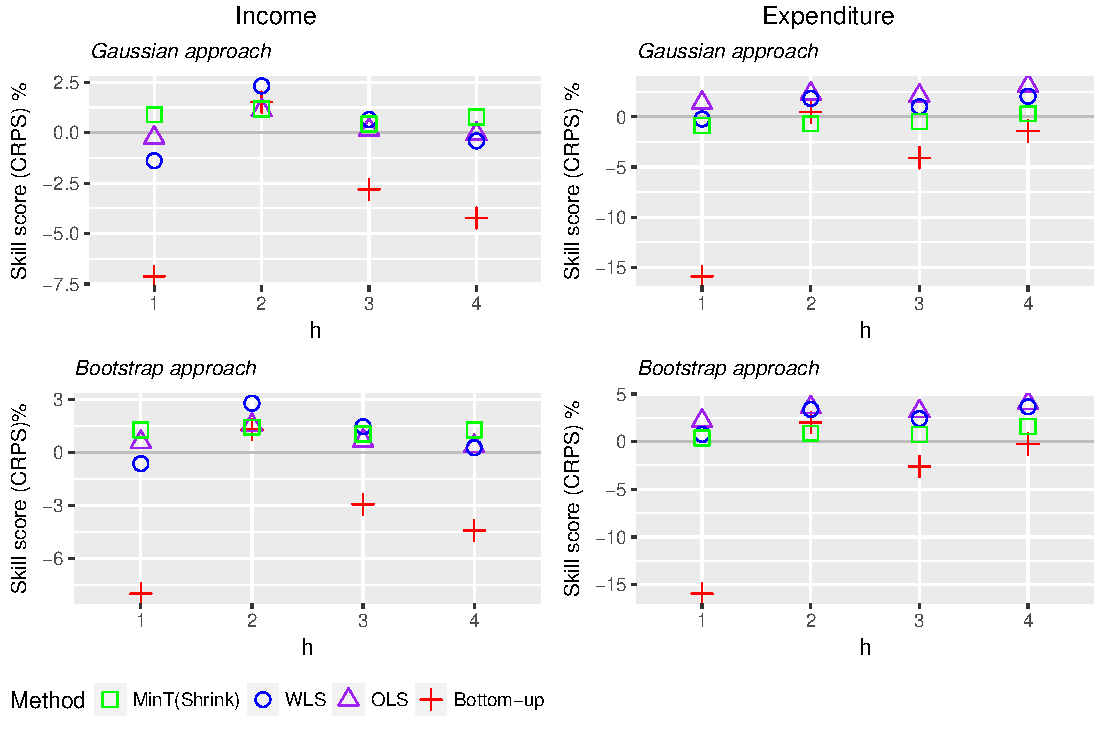
\includegraphics[width=\textwidth]{Figs/Results/ProbF_UnivS.pdf}
	\caption{Skill scores for probabilistic forecasts of top-level GDP from different reconciliation methods (with reference to base forecasts) using CRPS. Top panels refer to the results for Gaussian approach and bottom panels refer to the non-parametric bootstrap approach. The left panel refers to the income hierarchy and the right panel to the expenditure hierarchy.}
	\label{fig: Prob-forecasts-SS_CRPS}
\end{figure}

We now turn our attention towards results for probabilistic forecasts. \autoref{fig: Prob-forecasts-SS_ES} shows results for the energy score which as a multivariate score summarises forecast accuracy over the entire hierarchy. Once again all results are presented as skill scores relative to base forecasts. The top panels refer to results assuming Gaussian probabilistic forecasts as described in \autoref{sec:probrecgauss} while the bottom panels refer to the non-parametric bootstrap method described in \autoref{sec:probrecnp}. The left panels correspond to the income hierarchy while the right panels correspond to the expenditure hierarchy. For the income hierarchy, all methods improve upon base forecasts at all horizons. In nearly all cases the best performing reconciliation method is MinT(Shrink), a notable result since the optimal properties for MinT have thus far only been established theoretically in the point forecasting case. For the larger expenditure hierarchy results are little more mixed. While bottom-up tends to perform poorly, all reconciliation methods improve upon base forecasts (with the single exception of MinT(Shrink) in the Gaussian framework four quarters ahead). Interestingly, OLS performs best under the assumption of Gaussianity --- this may indicate that OLS is a more robust method under model misspecification but further investigation is required.

Finally, \autoref{fig: Prob-forecasts-SS_CRPS} displays the skill scores based on the cumulative ranked probability score for a single series, namely top-level GDP\@. The cause of the poor performance of bottom-up reconciliation as a failure to accurately forecast aggregate series is apparent here.

\section{Conclusions}\label{sec:conclusions}

In the macroeconomic setting, we have demonstrated the potential for forecast reconciliation methods to not only provide coherent forecasts, but to also improve overall forecast accuracy. This result holds for both point forecasts and probabilistic forecasts, for the two different hierarchies we consider and over different forecasting horizons. Even where the objective is to only forecast a single series, for instance top-level GDP, the application of forecast reconciliation methods improves forecast accuracy.

By comparing results from different forecast reconciliation techniques we draw a number of conclusions. Despite its simplicity, the single-level bottom-up approach can perform poorly at more aggregated levels of the hierarchy. Meanwhile, when forecast accuracy at the bottom level is evaluated, OLS tends to break down in some instances. Overall, the WLS and MinT(Shrink) methods (and particularly the latter) tend to yield the highest improvements in forecast accuracy. Similar results can be found in both simulations and the empirical studies of \citet{AthEtAl2017} and \citet{WicEtAl2019}.

There are a number of open avenues for research in the literature on forecast reconciliation, some of which are particularly relevant to macroeconomic applications. First there is scope to consider more complex aggregation structures, for instance in addition to the hierarchies we have already considered, data on GDP and GDP components disaggregated along geographical lines are also available. This leads to a grouped aggregation structure. Also, given the substantial literature on the optimal frequency at which to analyse macroeconomic data, a study on forecasting GDP or other variables as a temporal hierarchy may be of interest. In this chapter we have only shown that reconciliation methods can be used to improve forecast accuracy when univariate ARIMA models are used to produce base forecasts. It will be interesting to evaluate whether such results hold when a multivariate approach, e.g.\ a Bayesian VAR or dynamic factor model, is used to generate base forecasts, or whether the gains from forecast reconciliation would be more modest. Finally, a current limitation of the forecast reconciliation literature is that it only applies to collections of time series that adhere to linear constraints. In macroeconomics there are many examples of data that adhere to non-linear constraints, for instance real GDP is a complicated but deterministic function of GDP components and price deflators. The extension of forecast reconciliation methods to non-linear constraints potentially holds great promise for continued improvement in macroeconomic forecasting.

\clearpage

\bibliographystyle{agsm}
\bibliography{References_BookChapter_HTS}

\clearpage

\section*{Appendix}
\addcontentsline{toc}{section}{Appendix 1}

\begin{table}[!h]
	\caption{Variables, Series IDs and their descriptions for the Income approach}
	\small
	\centering
	\begin{tabular*}{\columnwidth}[width = \textwidth]{lll}
		\toprule
		\textbf{Variable} & \textbf{Series ID} & \textbf{Description}\\
		\midrule
    Gdpi            & A2302467A & GDP(I)\\
    Sdi             & A2302413V & Statistical discrepancy (I)\\
    Tsi             & A2302412T & Taxes less subsidies (I)\\
    TfiCoeWns       & A2302399K & Compensation of employees; Wages and salaries\\
    TfiCoeEsc       & A2302400J & Compensation of employees; Employers' social contributions\\
		\addlinespace
    TfiCoe          & A2302401K & Compensation of employees\\
    TfiGosCopNfnPvt & A2323369L & Private non-financial corporations; Gross operating surplus\\
    TfiGosCopNfnPub & A2302403R & Public non-financial corporations; Gross operating surplus\\
    TfiGosCopNfn    & A2302404T & Non-financial corporations; Gross operating surplus\\
    TfiGosCopFin    & A2302405V & Financial corporations; Gross operating surplus\\
		\addlinespace
    TfiGosCop       & A2302406W & Total corporations; Gross operating surplus\\
    TfiGosGvt       & A2298711F & General government; Gross operating surplus\\
    TfiGosDwl       & A2302408A & Dwellings owned by persons; Gross operating surplus\\
    TfiGos          & A2302409C & All sectors; Gross operating surplus\\
    TfiGmi          & A2302410L & Gross mixed income\\
    Tfi             & A2302411R & Total factor income\\
		\bottomrule
	\end{tabular*}
	\label{Tab: Income-hierarchy}
\end{table}

\begin{table}
	\caption{Variables, Series IDs and their descriptions for Expenditure Approach}
	\small
	\centering
	\begin{tabular*}{\columnwidth}[width = \textwidth]{lll}
		\toprule
		\textbf{Variable} & \textbf{Series ID} & \textbf{Description}\\
		\midrule
    Gdpe                  & A2302467A & GDP(E)\\
    Sde                   & A2302566J & Statistical Discrepancy(E)\\
    Exp                   & A2302564C & Exports of goods and services\\
    Imp                   & A2302565F & Imports of goods and services\\
    Gne                   & A2302563A & Gross national exp.\\
		\addlinespace
    GneDfdFceGvtNatDef    & A2302523J & Gen. gov. - National; Final consumption exp. - Defence\\
    GneDfdFceGvtNatNdf    & A2302524K & Gen. gov. - National; Final consumption exp. - Non-defence\\
    GneDfdFceGvtNat       & A2302525L & Gen. gov. - National; Final consumption exp.\\
    GneDfdFceGvtSnl       & A2302526R & Gen. gov. - State and local; Final consumption exp,\\
    GneDfdFceGvt          & A2302527T & Gen. gov.; Final consumption exp.\\
		\addlinespace
    GneDfdFce             & A2302529W & All sectors; Final consumption exp.\\
    GneDfdGfcPvtTdwNnu    & A2302543T & Pvt.; Gross fixed capital formation (GFCF)\\
    GneDfdGfcPvtTdwAna    & A2302544V & Pvt.; GFCF - Dwellings - Alterations and additions\\
    GneDfdGfcPvtTdw       & A2302545W & Pvt.; GFCF - Dwellings - Total\\
    GneDfdGfcPvtOtc       & A2302546X & Pvt.; GFCF - Ownership transfer costs\\
		\addlinespace
    GneDfdGfcPvtPbiNdcNbd & A2302533L & Pvt. GFCF - Non-dwelling construction - New building\\
    GneDfdGfcPvtPbiNdcNec & A2302534R & Pvt.; GFCF - Non-dwelling construction -\\
                          &           & New engineering construction\\
    GneDfdGfcPvtPbiNdcSha & A2302535T & Pvt.; GFCF - Non-dwelling construction -\\
                          &           & Net purchase of second hand \vphantom{1} assets\\
		\addlinespace
    GneDfdGfcPvtPbiNdc    & A2302536V & Pvt.; GFCF - Non-dwelling construction - Total\\
    GneDfdGfcPvtPbiNdmNew & A2302530F & Pvt.; GFCF - Machinery and equipment - New\\
    GneDfdGfcPvtPbiNdmSha & A2302531J & Pvt.; GFCF - Machinery and equipment -\\
                          &           & Net purchase of second hand assets\\
    GneDfdGfcPvtPbiNdm    & A2302532K & Pvt.; GFCF - Machinery and equipment - Total\\
		\addlinespace
    GneDfdGfcPvtPbiCbr    & A2716219R & Pvt.; GFCF - Cultivated biological resources\\
    GneDfdGfcPvtPbiIprRnd & A2716221A & Pvt.; GFCF - Intellectual property products -\\
                          &           & Research and development\\
    GneDfdGfcPvtPbiIprMnp & A2302539A & Pvt.; GFCF - Intellectual property products -\\
                          &           & Mineral and petroleum exploration\\
		\addlinespace
    GneDfdGfcPvtPbiIprCom & A2302538X & Pvt.; GFCF - Intellectual property products - Computer software\\
    GneDfdGfcPvtPbiIprArt & A2302540K & Pvt.; GFCF - Intellectual property products - Artistic originals\\
    GneDfdGfcPvtPbiIpr    & A2716220X & Pvt.; GFCF - Intellectual property products Total\\
    GneDfdGfcPvtPbi       & A2302542R & Pvt.;  GFCF - Total private business investment\\
    GneDfdGfcPvt          & A2302547A & Pvt.; GFCF\\
		\addlinespace
    GneDfdGfcPubPcpCmw    & A2302548C & Plc. corporations - Commonwealth; GFCF\\
    GneDfdGfcPubPcpSnl    & A2302549F & Plc. corporations - State and local; GFCF\\
    GneDfdGfcPubPcp       & A2302550R & Plc. corporations; GFCF Total\\
    GneDfdGfcPubGvtNatDef & A2302551T & Gen. gov. - National; GFCF - Defence\\
    GneDfdGfcPubGvtNatNdf & A2302552V & Gen. gov. - National ; GFCF - Non-defence\\
		\addlinespace
    GneDfdGfcPubGvtNat    & A2302553W & Gen. gov. - National ; GFCF Total\\
    GneDfdGfcPubGvtSnl    & A2302554X & Gen. gov. - State and local; GFCF\\
    GneDfdGfcPubGvt       & A2302555A & Gen. gov.; GFCF\\
    GneDfdGfcPub          & A2302556C & Plc.; GFCF\\
    GneDfdGfc             & A2302557F & All sectors; GFCF\\
		\bottomrule
	\end{tabular*}
	\label{Tab:Expenditure-hierarchy-1}
\end{table}

\begin{table}[h]
	\caption{Variables, Series IDs and their descriptions for Changes in Inventories - Expenditure Approach}
	\small
	\centering
	\begin{tabular*}{\columnwidth}[width = \textwidth]{lll}
		\toprule
		\textbf{Variable} & \textbf{Series ID} & \textbf{Description}\\
		\midrule
    GneCii       & A2302562X  & Changes in Inventories\\
    GneCiiPfm    & A2302560V  & Farm\\
    GneCiiPba    & A2302561W  & Public authorities\\
    GneCiiPnf    & A2302559K  & Private; Non-farm Total\\
    GneCiiPnfMin & A83722619L & Private; Mining (B)\\
		\addlinespace
    GneCiiPnfMan & A3348511X  & Private; Manufacturing (C)\\
    GneCiiPnfWht & A3348512A  & Private; Wholesale trade (F)\\
    GneCiiPnfRet & A3348513C  & Private; Retail trade (G)\\
    GneCiiPnfOnf & A2302273C  & Private; Non-farm; Other non-farm industries\\
		\bottomrule
	\end{tabular*}
	\label{Tab:Expenditure-hierarchy-2}
\end{table}

\begin{table}
	\caption{Variables, Series IDs and their descriptions for Household Final Consumption - Expenditure Approach}
	\small
	\centering
	\begin{tabular*}{\columnwidth}[width = \textwidth]{lll}
		\toprule
		\textbf{Variable} & \textbf{Series ID} & \textbf{Description}\\
		\midrule
    GneDfdHfc          & A2302254W & Household Final Consumption Expenditure\\
    GneDfdFceHfcFud    & A2302237V & Food\\
    GneDfdFceHfcAbt    & A3605816F & Alcoholic beverages and tobacco\\
    GneDfdFceHfcAbtCig & A2302238W & Cigarettes and tobacco\\
    GneDfdFceHfcAbtAlc & A2302239X & Alcoholic beverages\\
		\addlinespace
    GneDfdFceHfcCnf    & A2302240J & Clothing and footwear\\
    GneDfdFceHfcHwe    & A3605680F & Housing, water, electricity, gas and other fuels\\
    GneDfdFceHfcHweRnt & A3605681J & Actual and imputed rent for housing\\
    GneDfdFceHfcHweWsc & A3605682K & Water and sewerage charges\\
    GneDfdFceHfcHweEgf & A2302242L & Electricity, gas and other fuel\\
		\addlinespace
    GneDfdFceHfcFhe    & A2302243R & Furnishings and household equipment\\
    GneDfdFceHfcFheFnt & A3605683L & Furniture, floor coverings and household goods\\
    GneDfdFceHfcFheApp & A3605684R & Household appliances\\
    GneDfdFceHfcFheTls & A3605685T & Household tools\\
    GneDfdFceHfcHlt    & A2302244T & Health\\
		\addlinespace
    GneDfdFceHfcHltMed & A3605686V & Medicines, medical aids and therapeutic appliances\\
    GneDfdFceHfcHltHsv & A3605687W & Total health services\\
    GneDfdFceHfcTpt    & A3605688X & Transport\\
    GneDfdFceHfcTptPvh & A2302245V & Purchase of vehicles\\
    GneDfdFceHfcTptOvh & A2302246W & Operation of vehicles\\
		\addlinespace
    GneDfdFceHfcTptTsv & A2302247X & Transport services\\
    GneDfdFceHfcCom    & A2302248A & Communications\\
    GneDfdFceHfcRnc    & A2302249C & Recreation and culture\\
    GneDfdFceHfcEdc    & A2302250L & Education services\\
    GneDfdFceHfcHcr    & A2302251R & Hotels, cafes and restaurants\\
		\addlinespace
    GneDfdFceHfcHcrCsv & A3605694V & Catering services\\
    GneDfdFceHfcHcrAsv & A3605695W & Accommodation services\\
    GneDfdFceHfcMis    & A3605696X & Miscellaneous goods and services\\
    GneDfdFceHfcMisOgd & A3605697A & Other goods\\
    GneDfdFceHfcMisIfs & A2302252T & Insurance and other financial services\\
    GneDfdFceHfcMisOsv & A3606485T & Other services\\
		\bottomrule
	\end{tabular*}
	\label{Tab:Expenditure-hierarchy-3}
\end{table}

\end{document}
